\chapter{\acf{camion}}

\section{Context}

\subsection{Motivation}

Uneven distributions of population and health-care providers lead to geographic disparity in accessibility for patients \cite{wang_why_2020}. For instance, Weiss et al. \cite{weiss_global_2020} showed that 8.9\% of the global population could not reach healthcare within one hour if they have access to motorized transport. In Germany, Bauer et al. \cite{bauer_spatial_2020} shown that 10\% of the population lived in areas with low accessibility for internal medicine and surgery. Location-allocation algorithms \cite{church_location_1999} can optimize the distribution and supply of health providers to reduce accessibility disparities. These algorithms seek the optimal placement of facilities for a desirable objective under certain constraints \cite{wang_measurement_2012}. For instance, Luo et al. developed an optimization algorithm to improve the healthcare planning in rural China by finding the best place and capacity for new health facilities \cite{luo_integrating_2014}. Tao et al. worked on a spatial optimization model to maximize equity in accessibility to residential care facility in Beijing, China \cite{tao_spatial_2014}. When optimizing health accessibility, there are two competing goals: equity and efficiency \cite{krugman_opinion_2013,meyer_equity_2008}. Equity may be defined as equal access to healthcare for everyone \cite{culyer_equity_1993}. An efficient situation is when everything has been done to help any person without harming anyone else \cite{hemenway_optimal_1982}. While some argue that efficiency should be ad-dressed in priority \cite{hemenway_optimal_1982}, others agree that equity is a matter of ethical obligation, especially in public health \cite{fried_rights_1975, oliver_equity_2004}.

\subsection{Location-allocation algorithms}

Regarding efficiency optimization, the most popular algorithms are p-median, \ac{lscp} and \ac{mclp}. The p-median algorithm minimizes the weighted sum of distances between users and facilities \cite{murad_using_2021}. \ac{lscp} minimizes the number of facilities needed to cover all demand \cite{shavandi_fuzzy_2006}. \ac{lscp} maximizes the demand covered within a desired distance or time threshold by locating a given number of facilities \cite{casado_heuristical_2005}.
To reach equal access to healthcare, quadratic programming has been used to  minimize the variance of accessibility scores defined by the \ac{2sfca} \cite{wang_planning_2013}. Similarly, a \ac{pso} algorithm was developed to minimize the total square difference between the accessibility score of each demand location and the weighted average accessibility score \cite{tao_spatial_2014}. Finally, a two-step optimization algorithm has been developed to address the dual objectives of efficiency and equality, by first choosing where to site new hospitals and then deciding which capacity they should have \cite{luo_two-step_2017,li_two-step_2017}.

\section{Methods}

However, most of the previous algorithms seek locations to open new health facilities. In this work, we are interested in the case where the health facilities are fixed, and the only lever to improve accessibility is to increase their capacities. Given a capacity budget, we want to know which facilities to grow and by how much. We introduce \ac{camion}, an accessibility optimization algorithm based on \ac{fca} and \ac{lp}. The initial accessibility score was computed with the \ac{e2sfca} algorithm \cite{luo_enhanced_2009} but our algorithm can generalize to more \ac{fca} derivatives.

\subsection{Overall optimization}

We model the problem as an optimization task. In our case, we want our optimization algorithm to find new care centers capacities given some constraints, so that the total accessibility is maximum. We apply optimization on a given region only, rather than on the whole metropolitan France. We chose this approach because healthcare planning is handled regionally rather than nationally. We show below that our optimization problem is a \ac{lp} problem.
In its standard form, \ac{lp} finds a vector $x$ that maximizes $c^T x$ under constraints $Ax \leq b$, where $A$ is a matrix and $b$ a vector. Boundaries can be set to $x$ such as $x \geq 0$. Consider $x_u$ the new capacity of a care center $u$, to be computed by the algorithm. Let $Q_u$ and $W_u$ be two vectors of size $m$, defined as follows:

\begin{align}
    Q_u &=  \sum_{s=1}^{r} W_s \sum_{i, d_{iu} \in I_s} P_i \\[10pt]
    W_u &=  \sum_{s=1}^{r} \sum_{i, d_{iu} \in I_s} W_s
\end{align}

We can compute the total accessibility as a sum on the m care centers:

\begin{align*}
    \sum_{i} A_i &= \sum_{i} \sum_{s=1}^{r} W_s \sum_{u, d_{iu} \in I_s} \frac{S_u}{Q_u} \\[10pt]
    \sum_{i} A_i &= \sum_{i} \sum_{i, d_{iu} \in I_s} W_s \frac{S_u}{Q_u} \\[10pt]
    \sum_{i} A_i &= \sum_{u} \frac{S_u}{Q_u} \sum_{s} \sum_{i, d_{iu}} W_s \\[10pt]
    \sum_{i} A_i &= \sum_{u} \frac{S_u}{Q_u} W_u \numberthis \label{eq:A_i_sum_u}
\end{align*}

\cref{eq:A_i_sum_u} can be rewritten in the \ac{lp} standard form with:

\begin{align*}
c &= \frac{W_u}{Q_u} \\
x_u &= S_u  \\
b &\geq \sum_{u} x_u  \\
x_{u_\text{min}} &\leq x_u \leq x_{u_\text{max}}
\end{align*}

The user-defined parameters are $b$, $x_{u_\text{min}}$ and $x_{u_\text{max}}$. $b$ is the total capacity to be shared across all the care centers. $x_{u_\text{min}}$ and $x_{u_\text{max}}$ are the capacity boundaries for care center $u$. If $b$ is set to the current total capacity, a care center can’t be grown unless another one is decreased. If $b > \sum_{u} x_u$, the capacity of care centers can be increased without decreasing other centers. We know how to solve \ac{lp} and we used the SciPy \cite{virtanen_scipy_2020} implementation of the revised simplex method as explained in \cite{bertsimas_introduction_1998}.
We now detail how we set the user-defined parameters to apply the \ac{lp} algorithm to our specific case. The additional capacity was set as +3\% of the overall activity of the region's care centers: $b = 1.03 \times \sum_{u} x_u$. The choice of the boundaries $x_{u_\text{min}}$  and $x_{u_\text{max}}$ is crucial and must be realistic. We studied the hospitals activity on the past four years (2016 to 2019) to retrieve the average growth percentage of a care center. The growth percentage is computed as follows: $(S_\text{2019} - S_\text{2016}) / S_\text{2016}$ . Among the care centers that grew and who had an existing oncology activity, the mean growth percentage was 23\%. Hence, we set $x_{u_\text{max}}$ as +20\% of the care center capacity. Regarding $x_{u_\text{min}}$, we set the boundary based on the cluster of the care center. For the three most specialized clusters, we set their $x_{u_\text{min}}$ equal to their current activity. We did this to prevent the algorithm from decreasing the most specialized and well-equipped care centers. Regarding the care centers from the other clusters, $x_{u_\text{min}}$, so that they could be emptied if need be. Finally, we set $x_{u_\text{max}}$ if the care center belongs to the least specialized cluster. The new capacities are indicative and should be further investigated to make sure they are relevant. Especially when setting an existing oncology activity to 0.

\subsection{Maxi-min optimization}

We now want to maximize the minimum accessibility. Let $z$ be that minimum accessibility.  Let $x_u$ be the capacity increase for facility $u$, whose previous capacity was $S_u$:

\begin{align*}
z &= \underset{i=1, ..., n}{min} A_i \\
z &\leq A_i \; \text{for all} \; i=1,...,n \\
A_i &= \sum_{s=1}^{r} W_s \sum_{u,d_{iu} \in I_s} \frac{S_u + x_u}{Q_u}
\end{align*}

For all $i=1, ... ,n$:

\begin{align*}
z &\leq \sum_{s=1}^{r} W_s \sum_{u, d_{iu} \in I_s} \frac{S_u + x_u}{Q_u} \\
z - \sum_{s=1}^{r} W_s \sum_{u,d_{iu} \in I_s} \frac{x_u}{Q_u} &\leq \sum_{s=1}^{r} W_s \sum_{u,d_{iu} \in I_s} \frac{S_u}{Q_u}
\end{align*}

We can add these new $n$ equations as constraints to the optimization problem, as well as the other constraints. The Linear Programming problem is now framed as the maximization of $c^T x$ with $c=(1, ... ,0)$ and $x=(z, ... ,0)$, both of size $m+1$ with m the number of facilities. The constraints are:

For all $i=1, ... ,n$:

\begin{align*}
z - \sum_{s=1}^{r} W_s \sum_{u,d_{iu} \in I_s} \frac{x_u}{Q_u} &\leq \sum{s=1}^{r} W_s \sum_{u,d_{iu} \in I_s} \frac{S_u}/{Q_u} \\
\sum_{u} x_u &\leq b \; \text{for a given budget} \; b \\
x_{u_\text{min}} &\leq x_u \leq x_{u_\text{max}}
\end{align*}

\section{Results}

Since we focused on describing the accessibility situation in Provence-Alpes-Cote-d'Azur, we now present the outcomes of our optimization algorithm in this same region. The algorithm was run with the user-specified parameters stated in the Methods Section: we chose to increase the overall oncology activity in the region by 3\% (+3,221 activity) and capped care centers to a 20\% maximum growth. The median accessibility in the region went from 0.0093 to 0.0103, a 11.1\% increase. The results are shown on \cref{fig:optim-paca}. Map (A) displays the accessibility delta ($A_{i_\text{after}} - A_{i_\text{before}}$) as well as the care centers eligible to grow. Centers from cluster 8 were hidden since we considered that they couldn't provide any oncology activity. The algorithm identified a list of 26 care centers where the oncology activity could grow to maximize the total accessibility in the region. These centers are either public or private hospitals, primarily located in the Avignon and Gap areas. The care centers located in high accessibility areas near Marseille and Nice were ignored by the algorithm because improving these zones is not a priority. The care center that grew the most is Clinique Sainte Catherine, in Avignon. Interestingly, this care center was recently bought by the Unicancer group, which coordinates all the cancer centers in France. This hospital's type will change to become a new \ac{clcc}. Thus, it is expected to grow in the next years and to be equipped with more oncology services and staff.

\begin{figure}[H]
    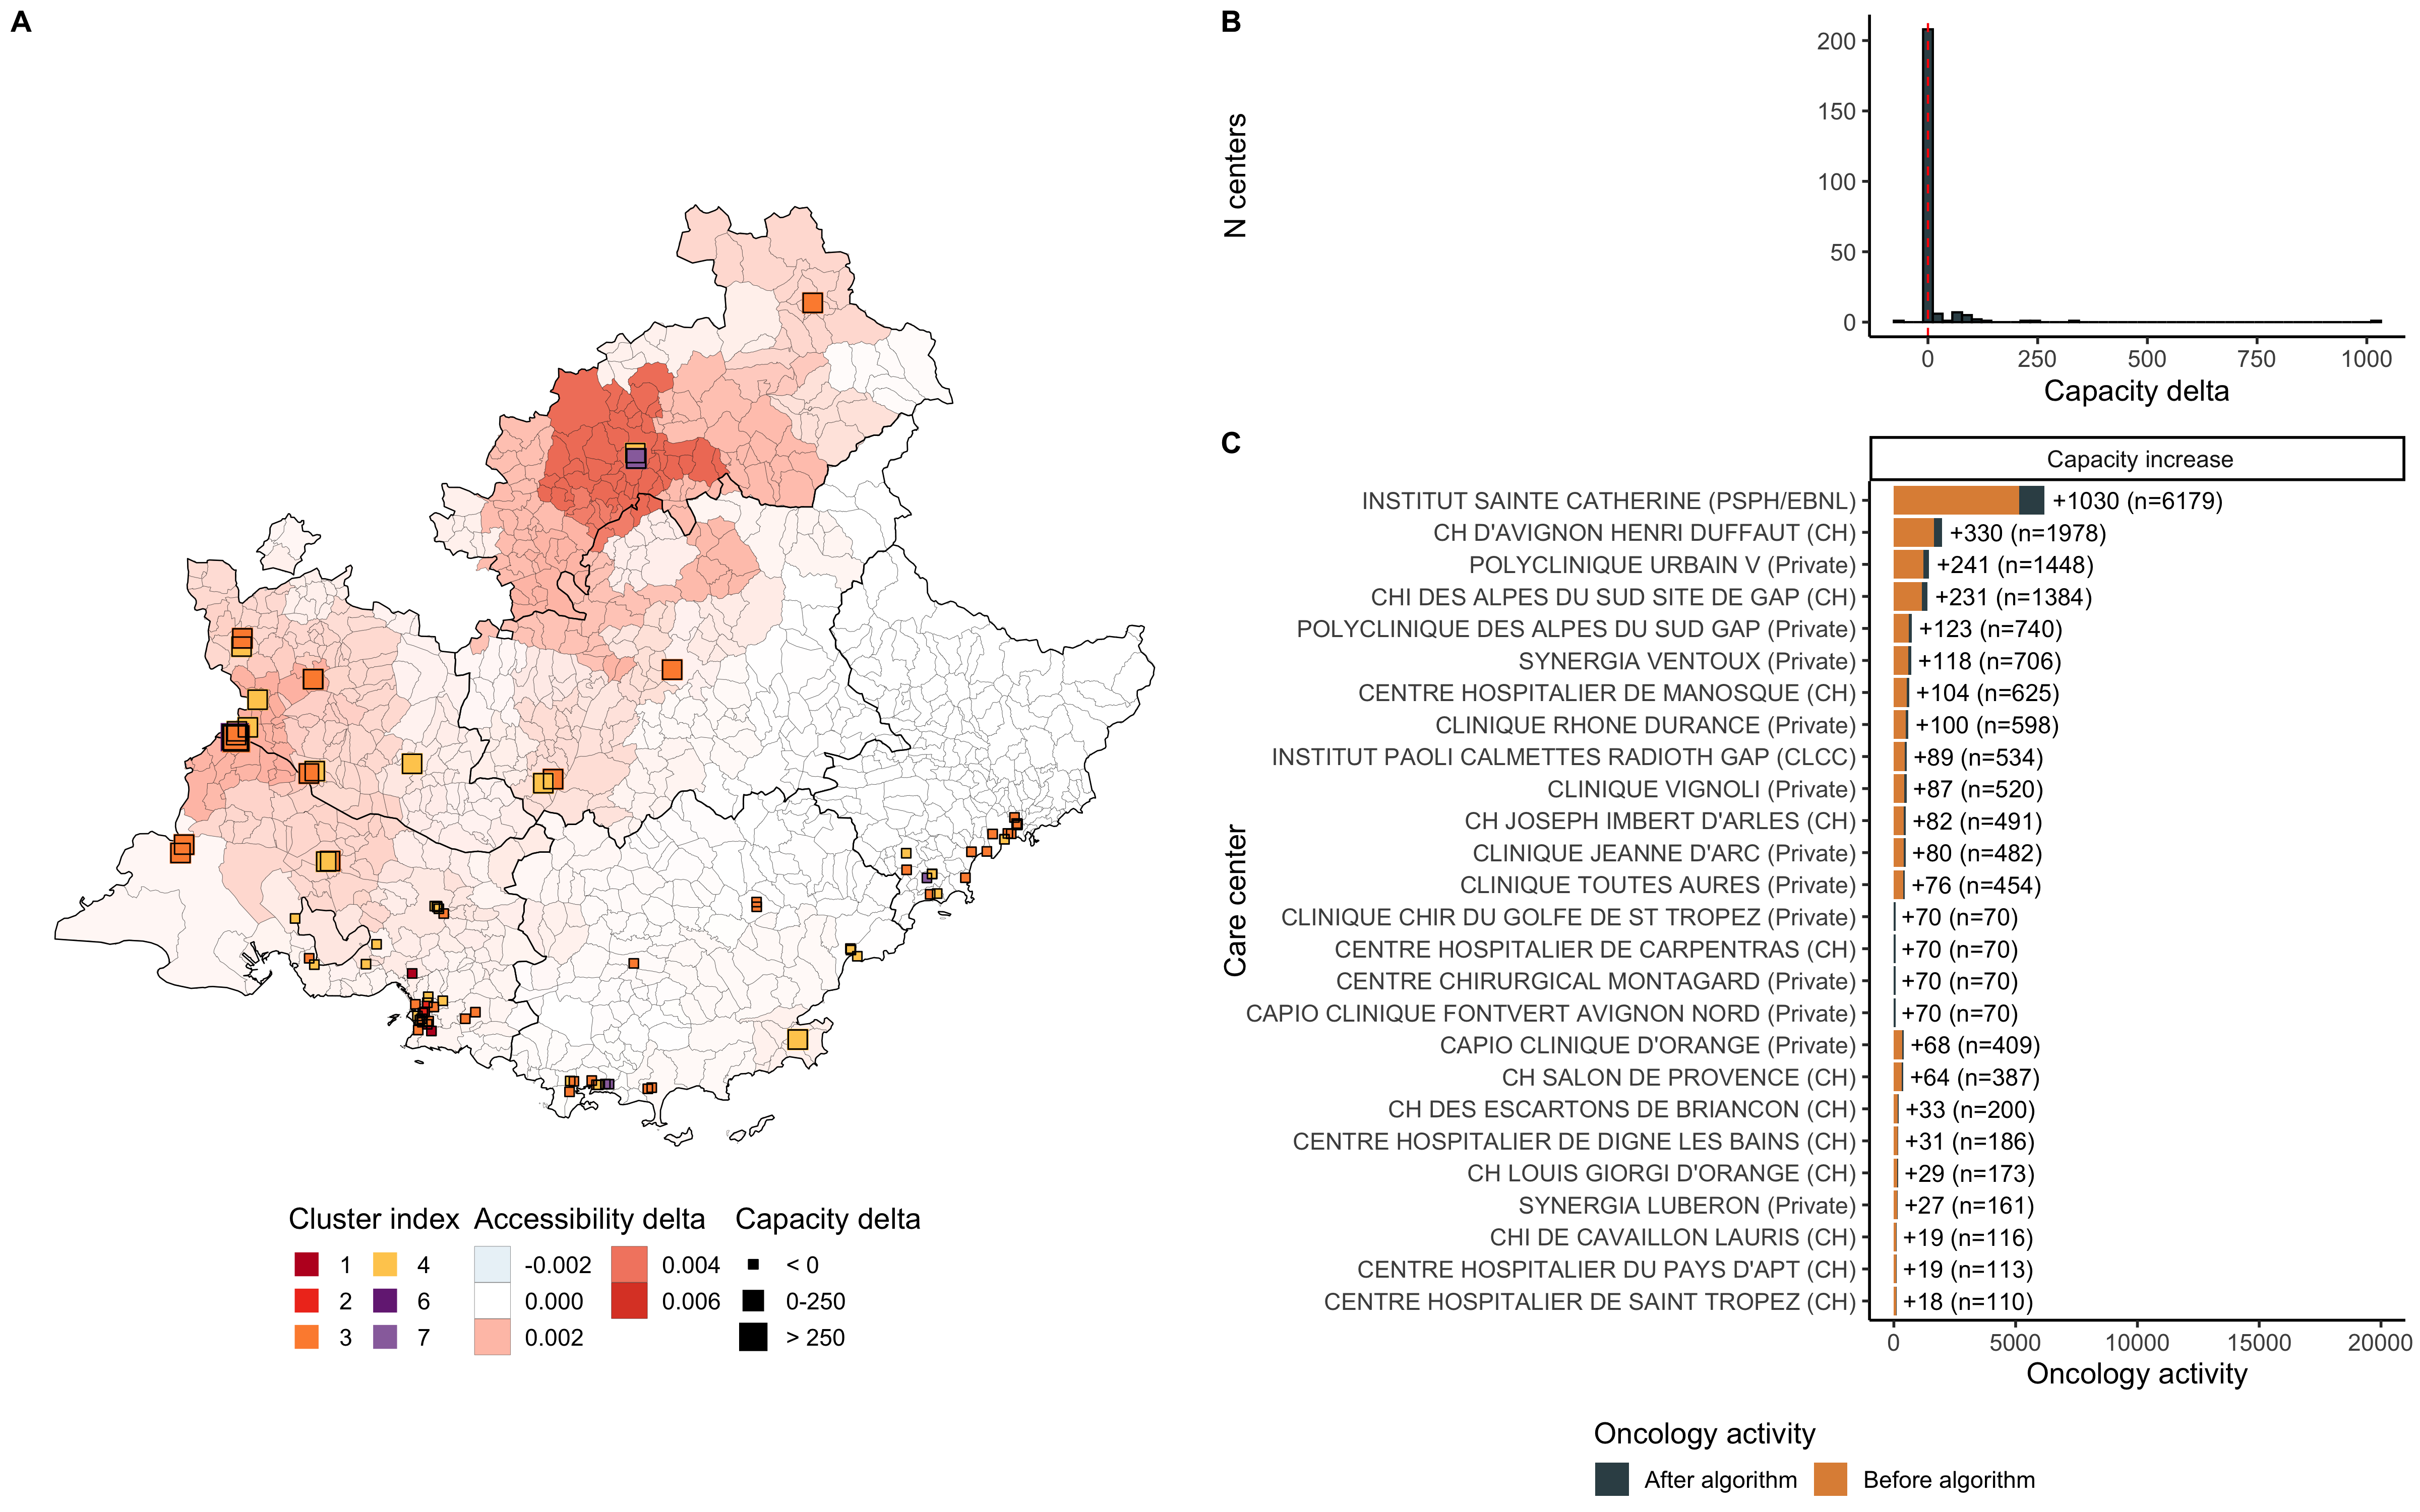
\includegraphics[width=0.9\textwidth]{images/camion/fig5_Provence-Alpes-Cote-d'Azur.png}
    \centering
    \caption{
        \textbf{Accessibility delta in Provence-Alpes-Cote-d'Azur region after running the optimization algorithm.} Map (A) displays the accessibility delta ($A_{i_\text{after}} - A_{i_\text{before}}$) by municipality. Plot (B) shows the capacity delta ($S_{u_\text{after}}-S_{u_\text{before}}$) distribution. Capacity was defined as the oncology activity: the number of patients with chemotherapy or radiotherapy and the number of medical or surgery stays related to oncology. We show the list of the care centers that grew the most (C)  and by how much. For instance, the hospital Institut Sainte Catherine in Avignon, was assigned a +1,030 capacity, for a total of n=6,179. Additional activity was 3,221. 26 centers grew and 1 decreased. Median accessibility before optimization was 0.0093 and 0.0103 after, corresponding to a 11.1\% increase.  Accessibility increased around cities like Avignon and Gap. Care centers near Nice were left unchanged by the algorithm.
    }
    \label{fig:optim-paca}
\end{figure}

While we described the results in Provence-Alpes-Cote-d'Azur region, we ran the algorithm with similar parameters on every region in metropolitan France. We observe two types of optimization strategies. For most regions, the algorithm manages to find a couple of areas where the accessibility can be locally improved, like it did in Provence-Alpes-Cote-d'Azur near Gap and Avignon. However, for regions like Ile-de-France and Haut-de-France, the hospital capacity increase is more uniformly distributed across the region. Most of the time, the algorithm left un-touched the large care centers located in dense cities with good accessibilities. This can be explained by the relatively low value of the additional activity parameter: with a very large value of additional activity, every care center will grow. If we keep it low, the algorithm identifies in which areas hospital capacity should be increased in priority.

\subsection*{Pays de la Loire}

\begin{figure}[H]
    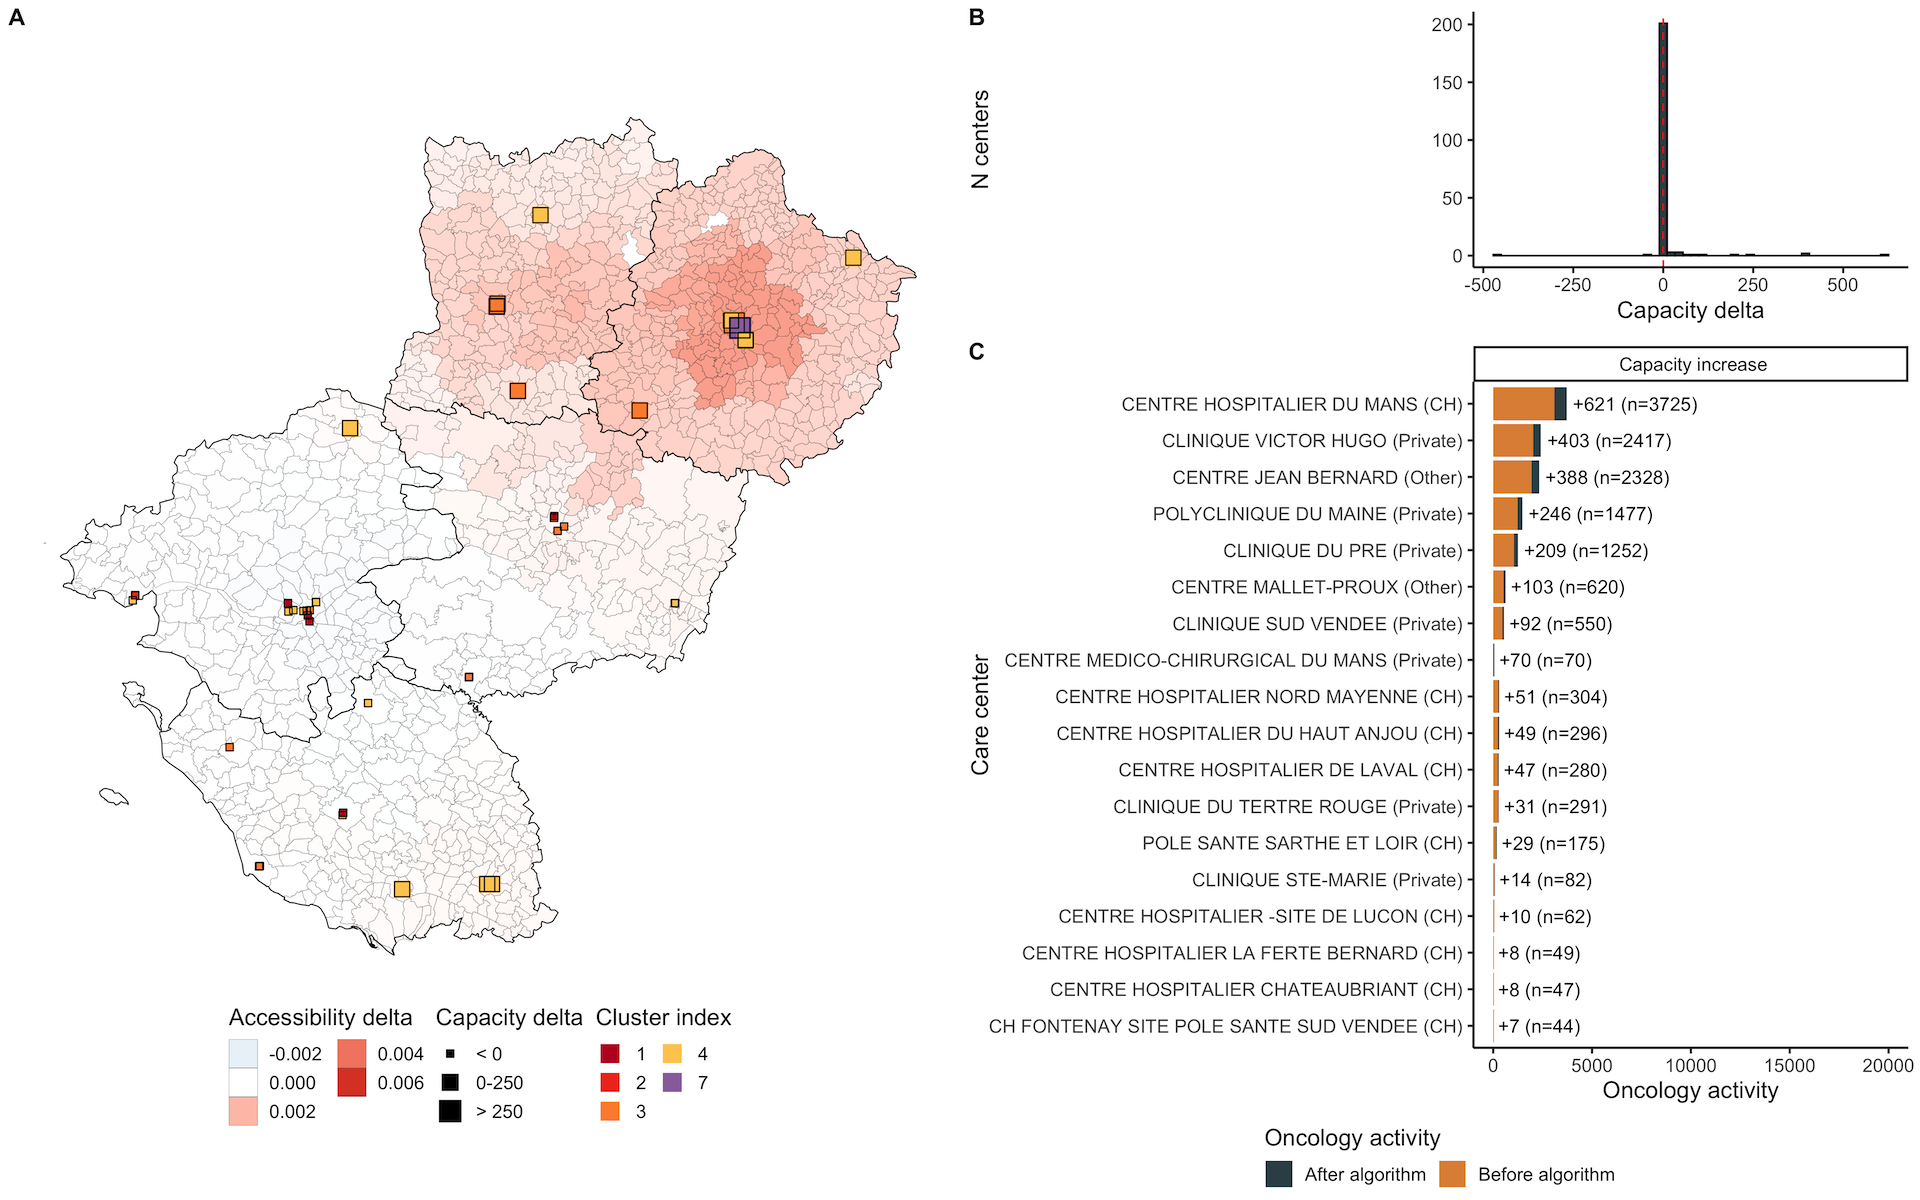
\includegraphics[width=0.9\textwidth]{images/camion/optim_region/optim_Pays-de-la-Loire.png}
    \centering
    \caption{
        \textbf{Optimization results in Pays-de-la-Loire.} Additional activity was 1,890. 18 centers grew and 2 decreased. Median accessibility before optimization was 0.0118 and 0.0121 after, corresponding to a 2.4\% increase. Accessibility grew near La Roche sur Yon, Angers and Le Mans.
    }
\end{figure}

\subsection*{Occitanie}

\begin{figure}[H]
    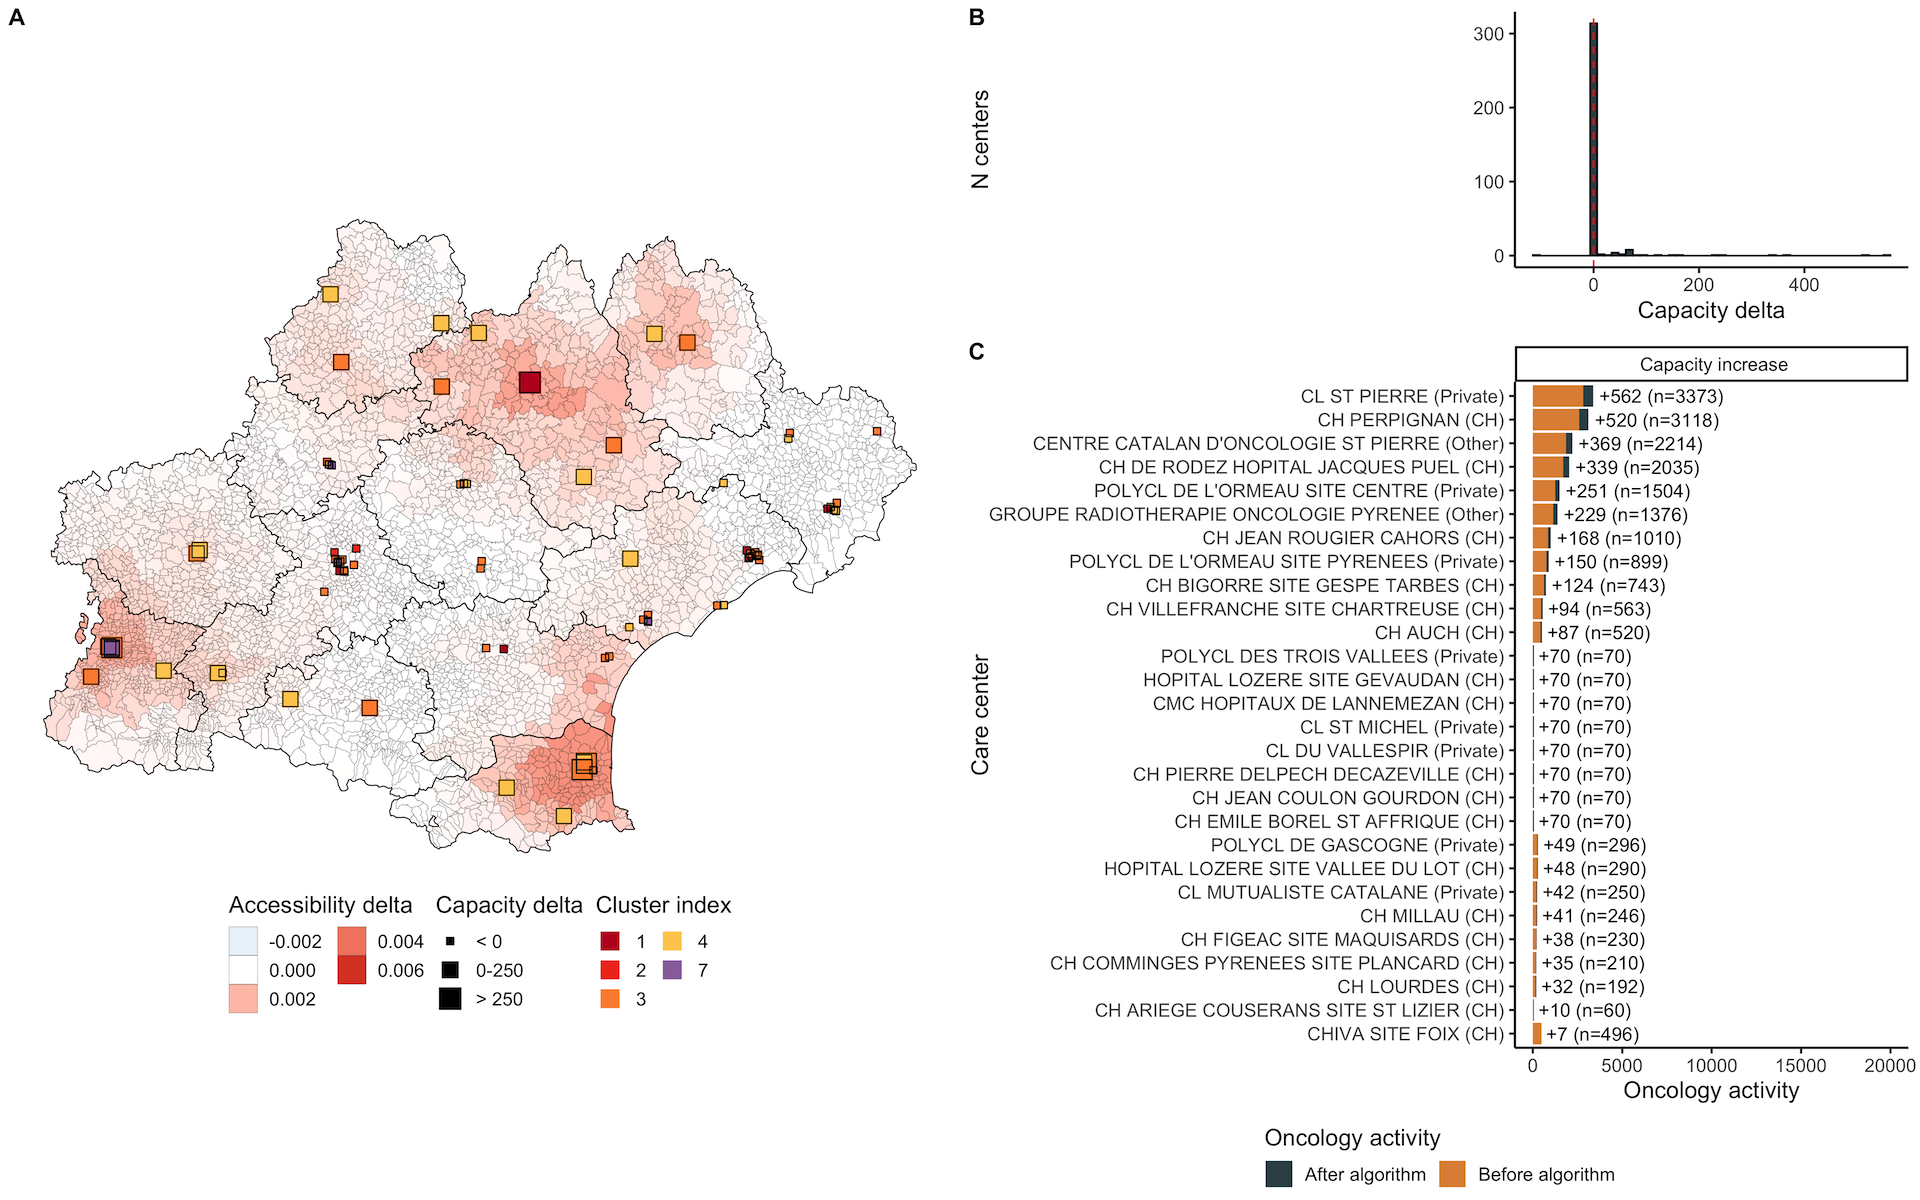
\includegraphics[width=0.9\textwidth]{images/camion/optim_region/optim_Occitanie.png}
    \centering
    \caption{
        \textbf{Optimization results in Occitanie.} Additional activity was 3,652. 28 centers grew and 1 decreased. Median accessibility before optimization was 0.0087 and 0.0091 after, corresponding to a 4.7\% increase. Accessibility grew around Perpignan, Rodez, Mende and Tarbes.
    }
\end{figure}

\subsection*{Nouvelle-Aquitaine}

\begin{figure}[H]
    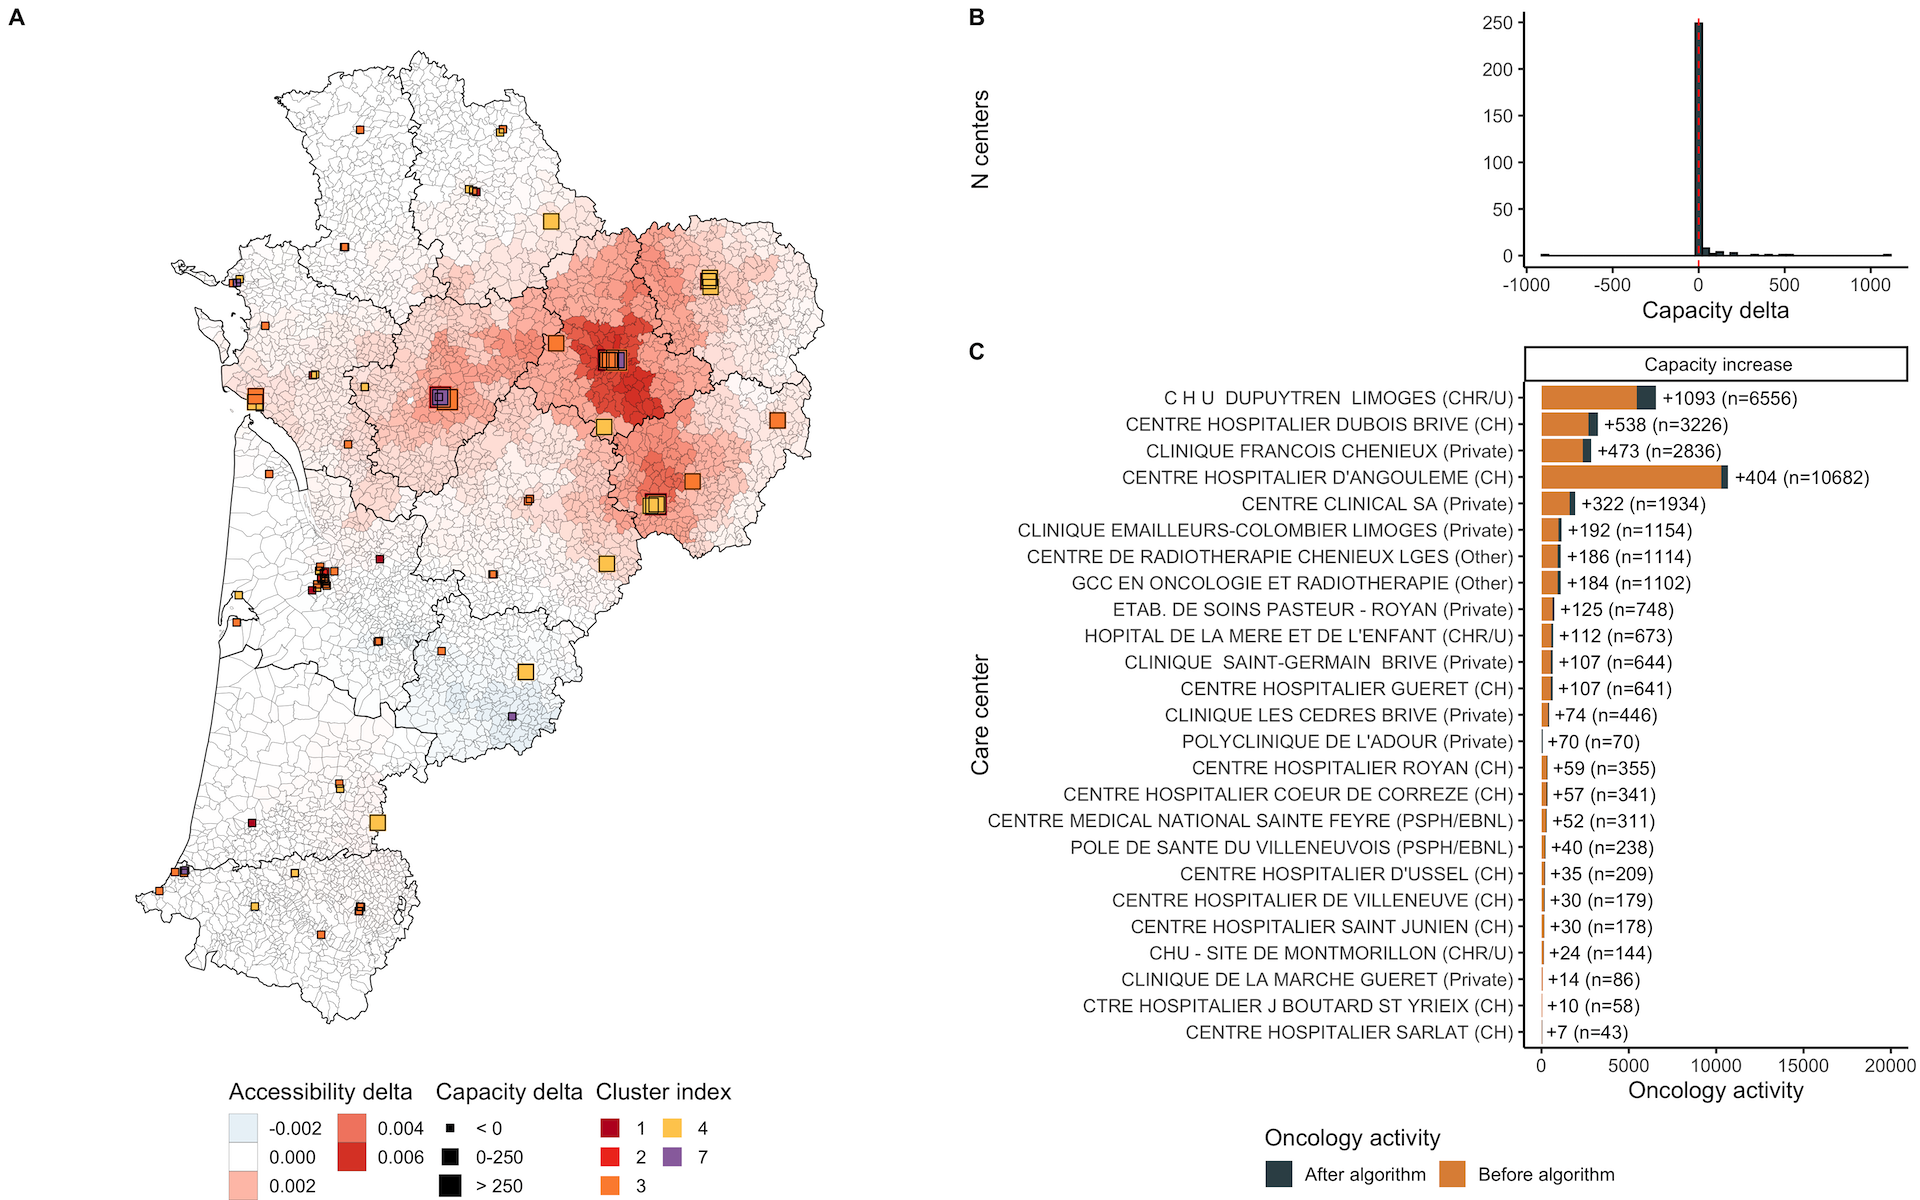
\includegraphics[width=0.9\textwidth]{images/camion/optim_region/optim_Nouvelle-Aquitaine.png}
    \centering
    \caption{
        \textbf{Optimization results in Nouvelle-Aquitaine.} Additional activity was 3,445. 25 centers grew and 1 decreased. Median accessibility before optimization was 0.0117 and 0.0119 after, corresponding to a 1.5\% increase. Accessibility grew around Limoges, Angouleme, and Brives-la-Gaillarde.
    }
\end{figure}

\subsection*{Normandie}

\begin{figure}[H]
    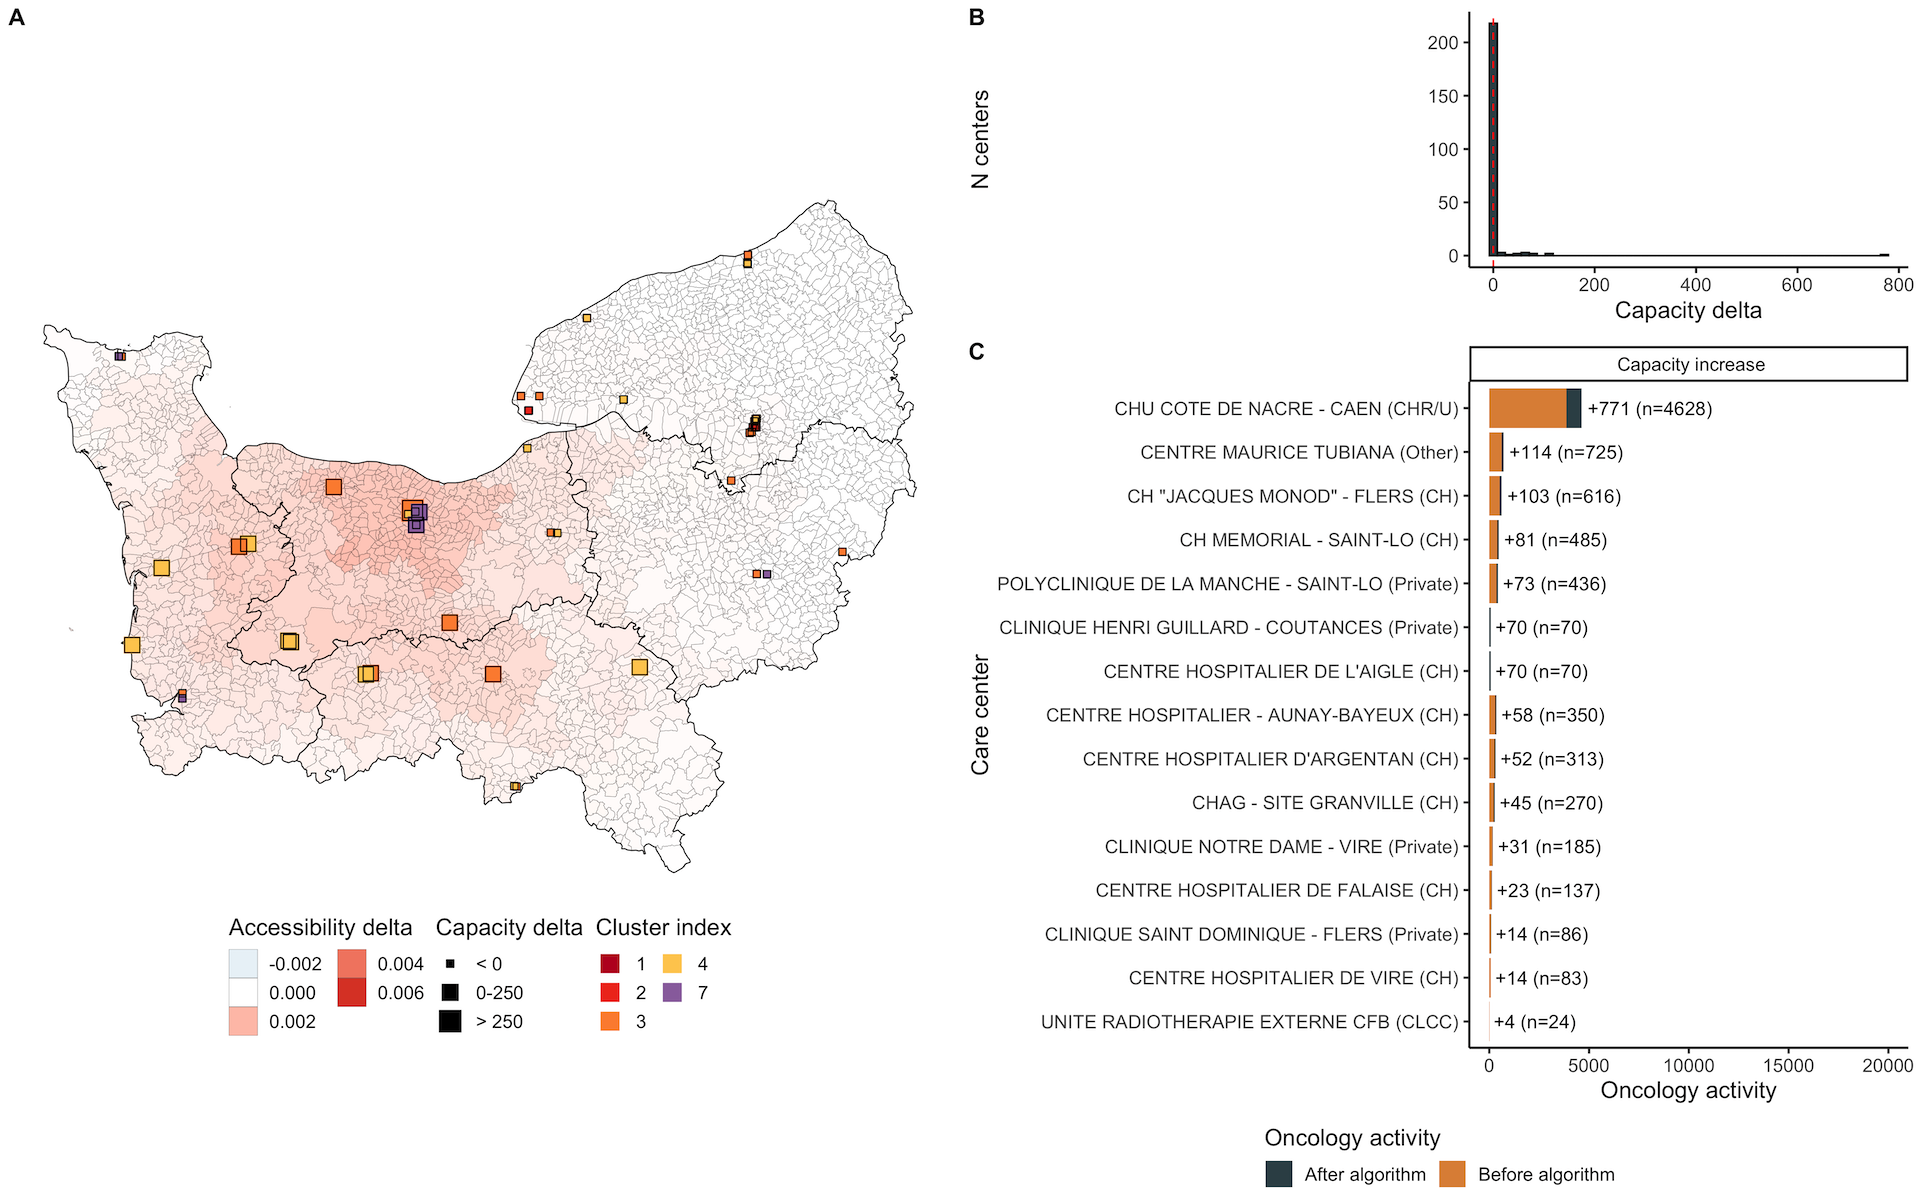
\includegraphics[width=0.9\textwidth]{images/camion/optim_region/optim_Normandie.png}
    \centering
    \caption{
        \textbf{Optimization results in Normandie.} Additional activity was 1,523. 15 centers grew and 0 decreased. Median accessibility before optimization was 0.0105 and 0.0106 after, corresponding to a 1\% increase. Accessibility grew near Caen, Argentan, and St-Lo.
    }
\end{figure}

\subsection*{Île-de-France}

\begin{figure}[H]
    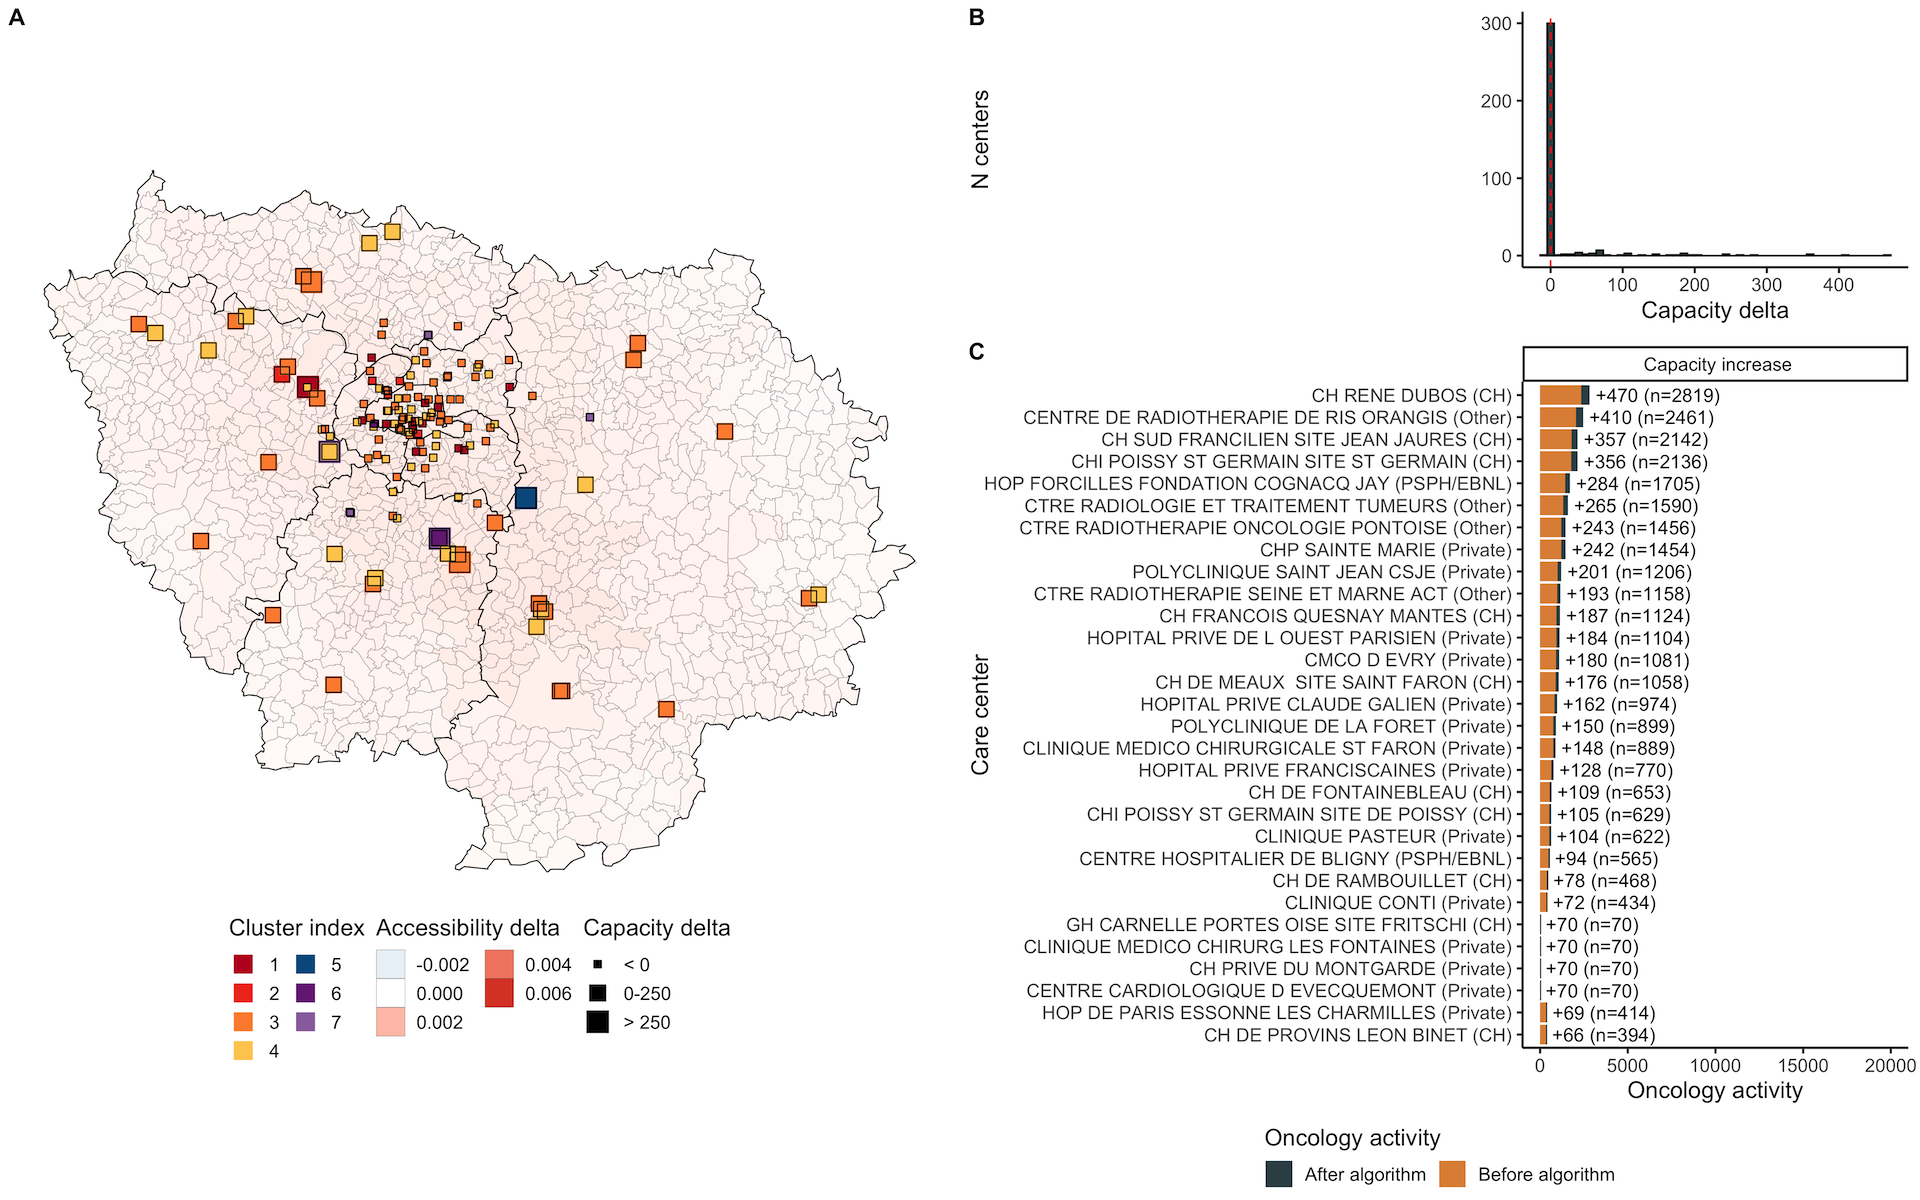
\includegraphics[width=0.9\textwidth]{images/camion/optim_region/optim_Ile-de-France.png}
    \centering
    \caption{
        \textbf{Optimization results in Ile-de-France.} Additional activity was 5,826. 44 centers grew and 1 decreased. Median accessibility before optimization was 0.0088 and 0.0089 after, corresponding to a 1.3\% increase. Accessibility grew around Mantes-la-Jolie, Rambouillet, Melun, and Evry.
    }
\end{figure}

\subsection*{Hauts-de-France}

\begin{figure}[H]
    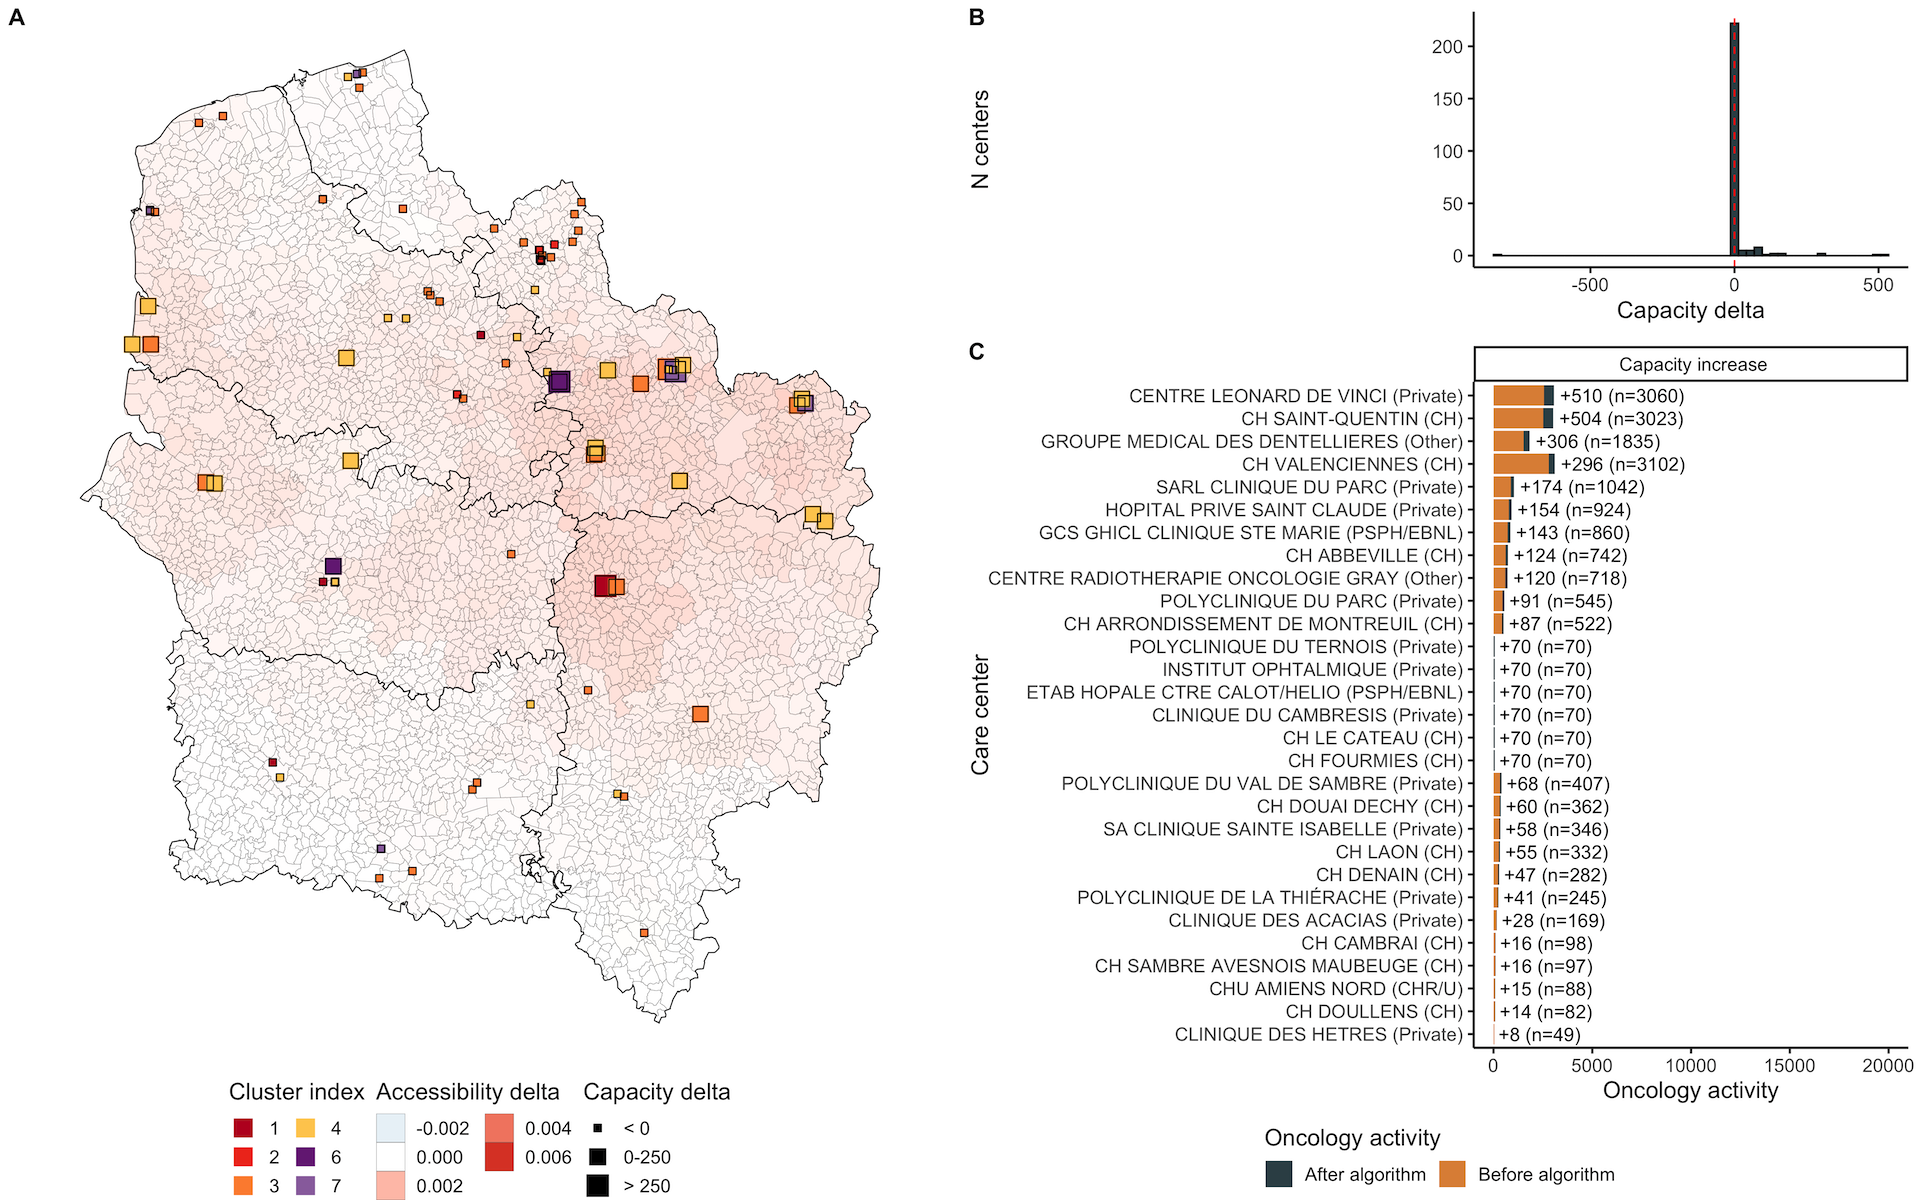
\includegraphics[width=0.9\textwidth]{images/camion/optim_region/optim_Hauts-de-France.png}
    \centering
    \caption{
        \textbf{Optimization results in Hauts-de-France.} Additional activity was 2,520. 29 centers grew and 1 decreased. Median accessibility before optimization was 0.01 and 0.0102 after, corresponding to a 2.1\% increase. Accessibility grew around St-Quentin and Valenciennes.
    }
\end{figure}

\subsection*{Grand Est}

\begin{figure}[H]
    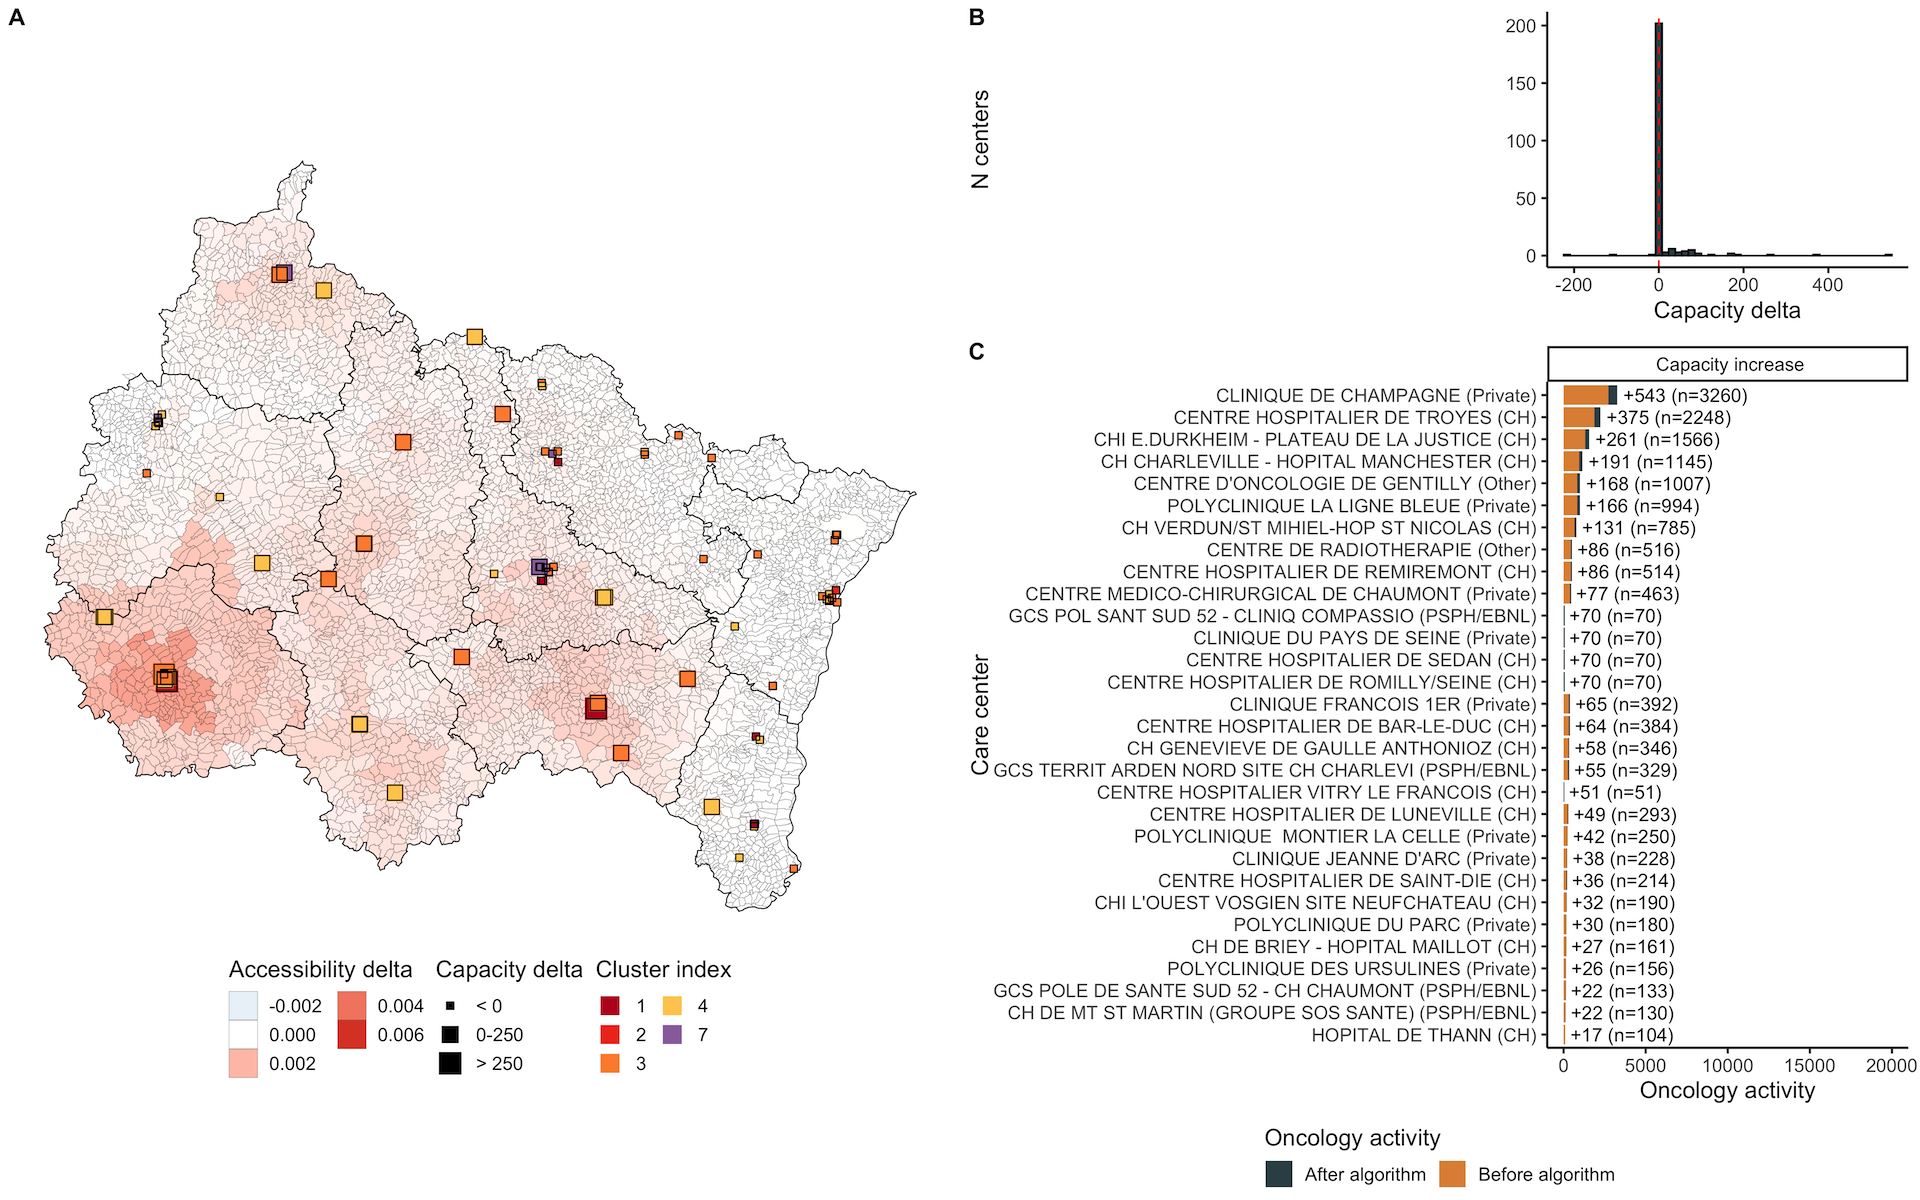
\includegraphics[width=0.9\textwidth]{images/camion/optim_region/optim_Grand-Est.png}
    \centering
    \caption{
        \textbf{Optimization results in Grand-Est.} Additional activity was 2,663. 31 centers grew and 4 decreased. Median accessibility before optimization was 0.0096 and 0.0099 after, corresponding to a 3\% increase. Accessibility grew around Troyes and Epinal.
    }
\end{figure}

\subsection*{Centre-Val de Loire}

\begin{figure}[H]
    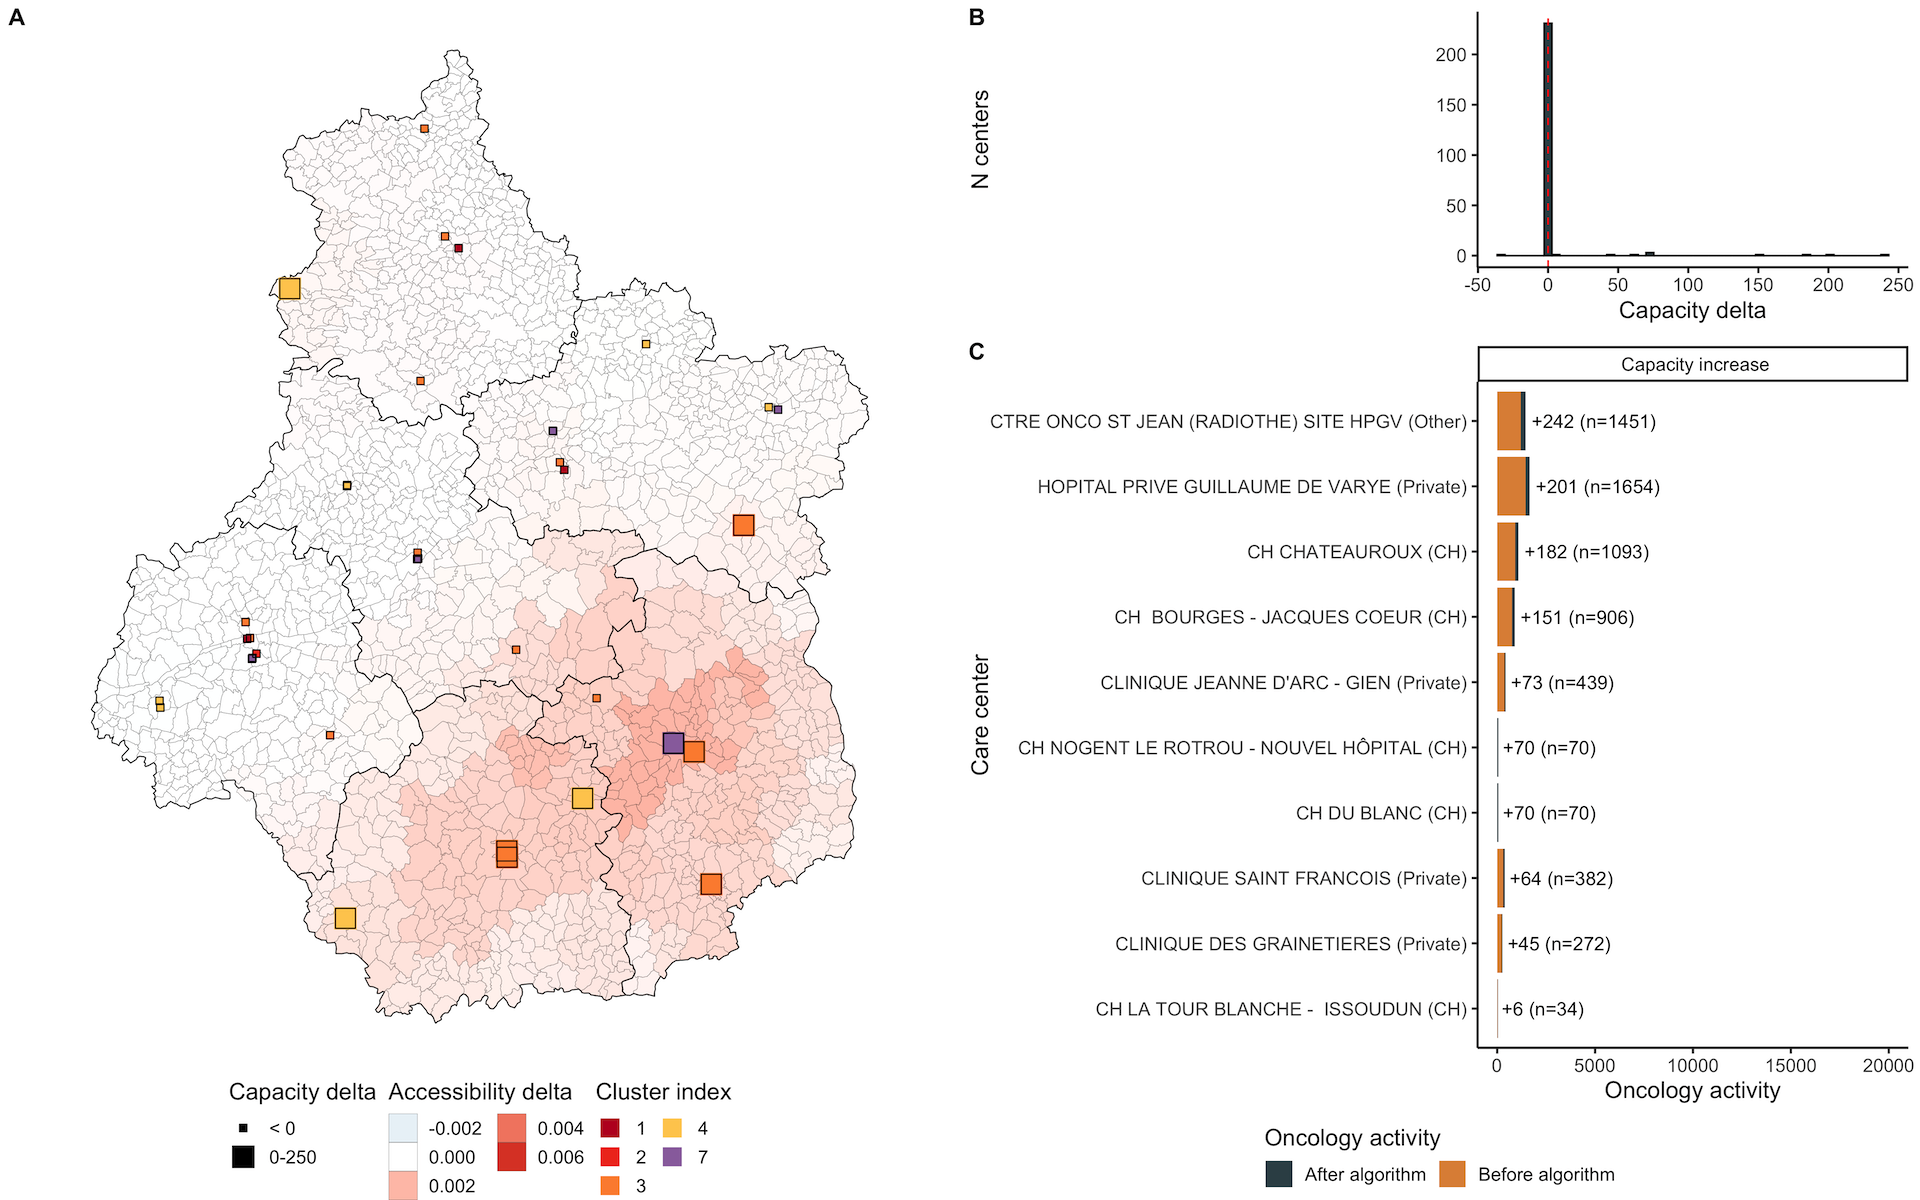
\includegraphics[width=0.9\textwidth]{images/camion/optim_region/optim_Centre-Val-de-Loire.png}
    \centering
    \caption{
        \textbf{Optimization results in Centre-Val-de-Loire.} Additional activity was 1,072. 10 centers grew and 1 decreased. Median accessibility before optimization was 0.0099 and 0.0102 after, corresponding to a 2.9\% increase. Accessibility grew around Tours, Blois, Bourges and Chateauroux.
    }
\end{figure}

\subsection*{Bretagne}

\begin{figure}[H]
    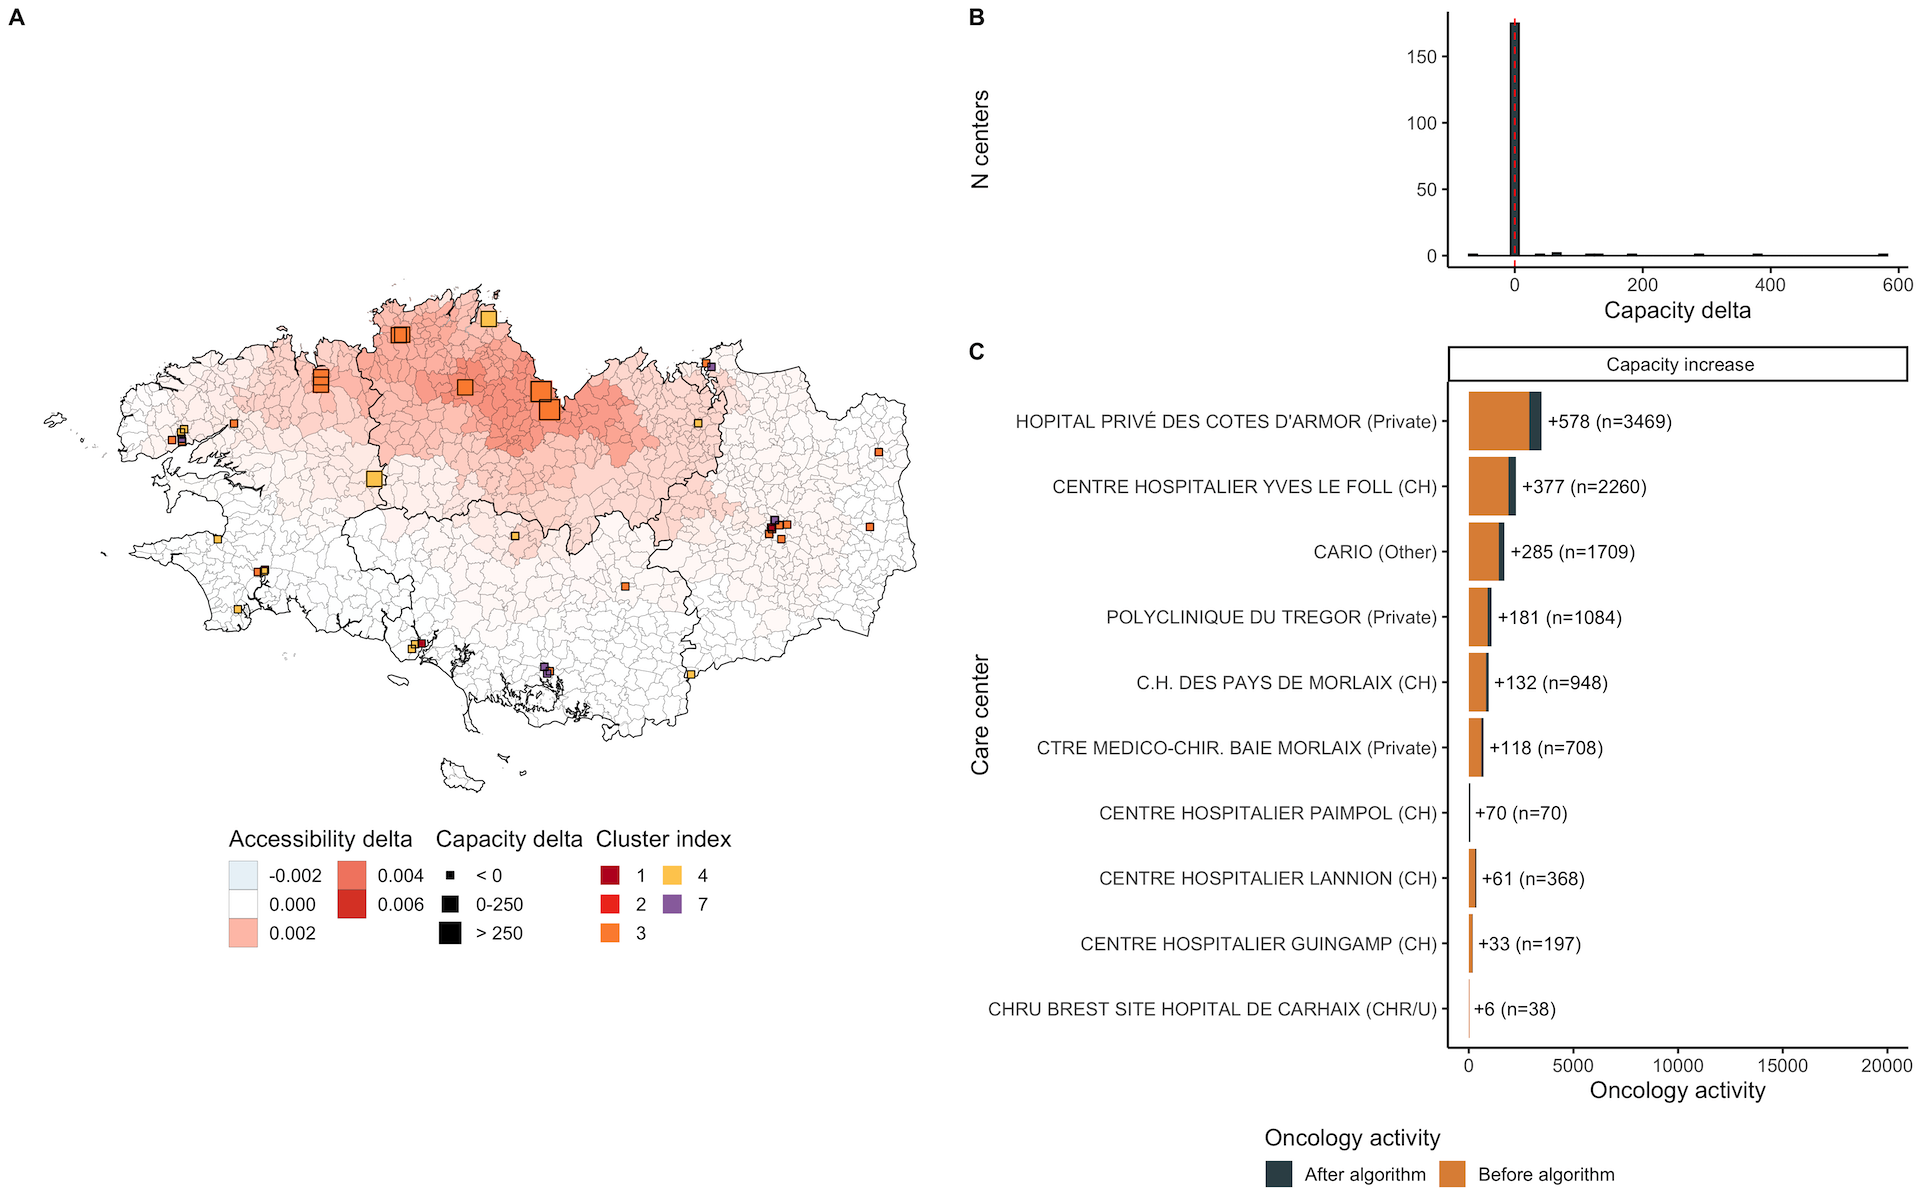
\includegraphics[width=0.9\textwidth]{images/camion/optim_region/optim_Bretagne.png}
    \centering
    \caption{
        \textbf{Optimization results in Bretagne.} Additional activity was 1,773. 10 centers grew and 2 decreased. Median accessibility before optimization was 0.0131 and 0.0134 after, corresponding to a 2.4\% increase. Accessibility grew around St-Brieuc and Quimper.
    }
\end{figure}

\subsection*{Bourgogne-Franche-Comté}

\begin{figure}[H]
    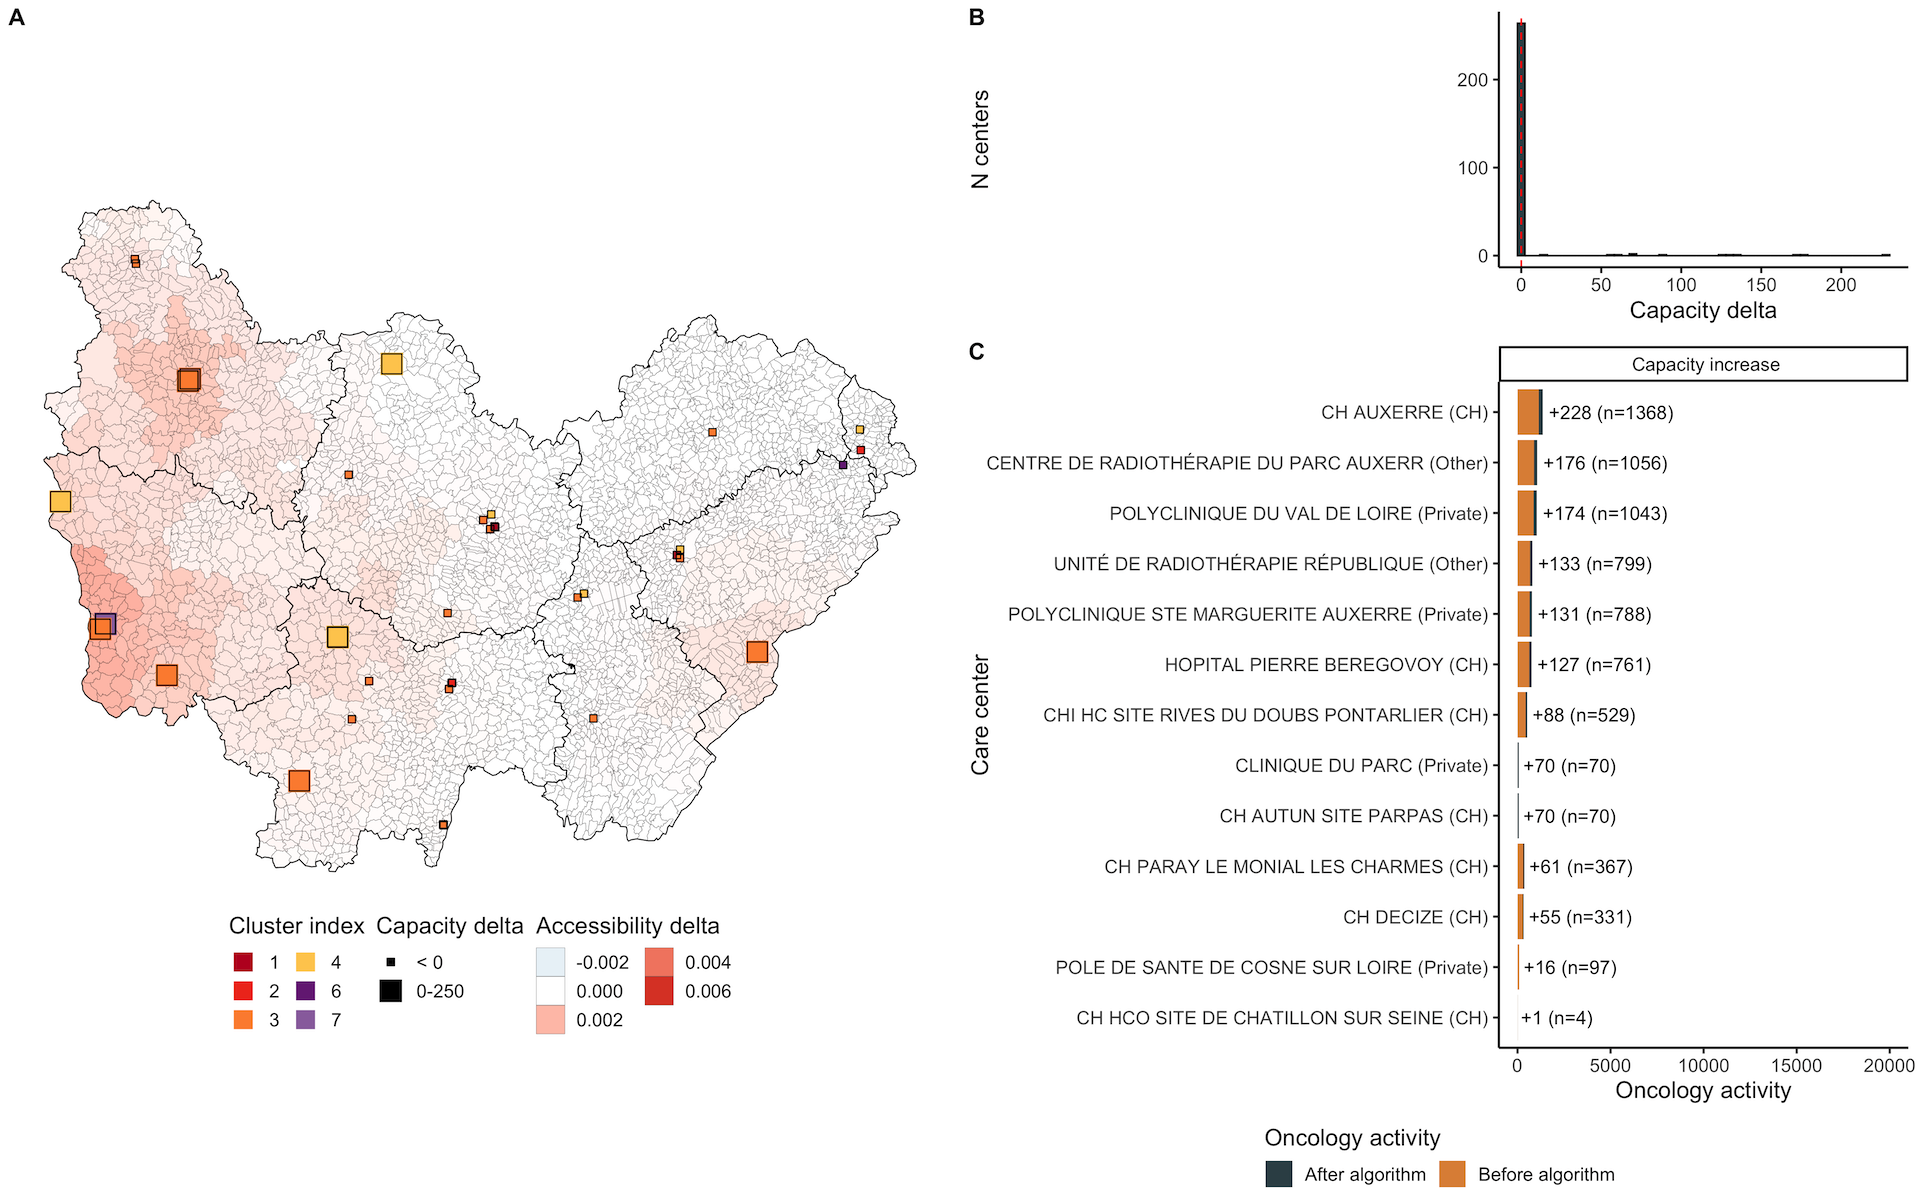
\includegraphics[width=0.9\textwidth]{images/camion/optim_region/optim_Bourgogne-Franche-Comte.png}
    \centering
    \caption{
        \textbf{Optimization results in Bourgogne-Franche-Comté.} Additional activity was 1,330. 13 centers grew and 0 decreased. Median accessibility before optimization was 0.0096 and 0.0098 after, corresponding to a 1.9\% increase. Accessibility grew around Nevers, Belfort, Vesoul and Auxerre.
    }
\end{figure}

\subsection*{Auvergne-Rhône-Alpes}

\begin{figure}[H]
    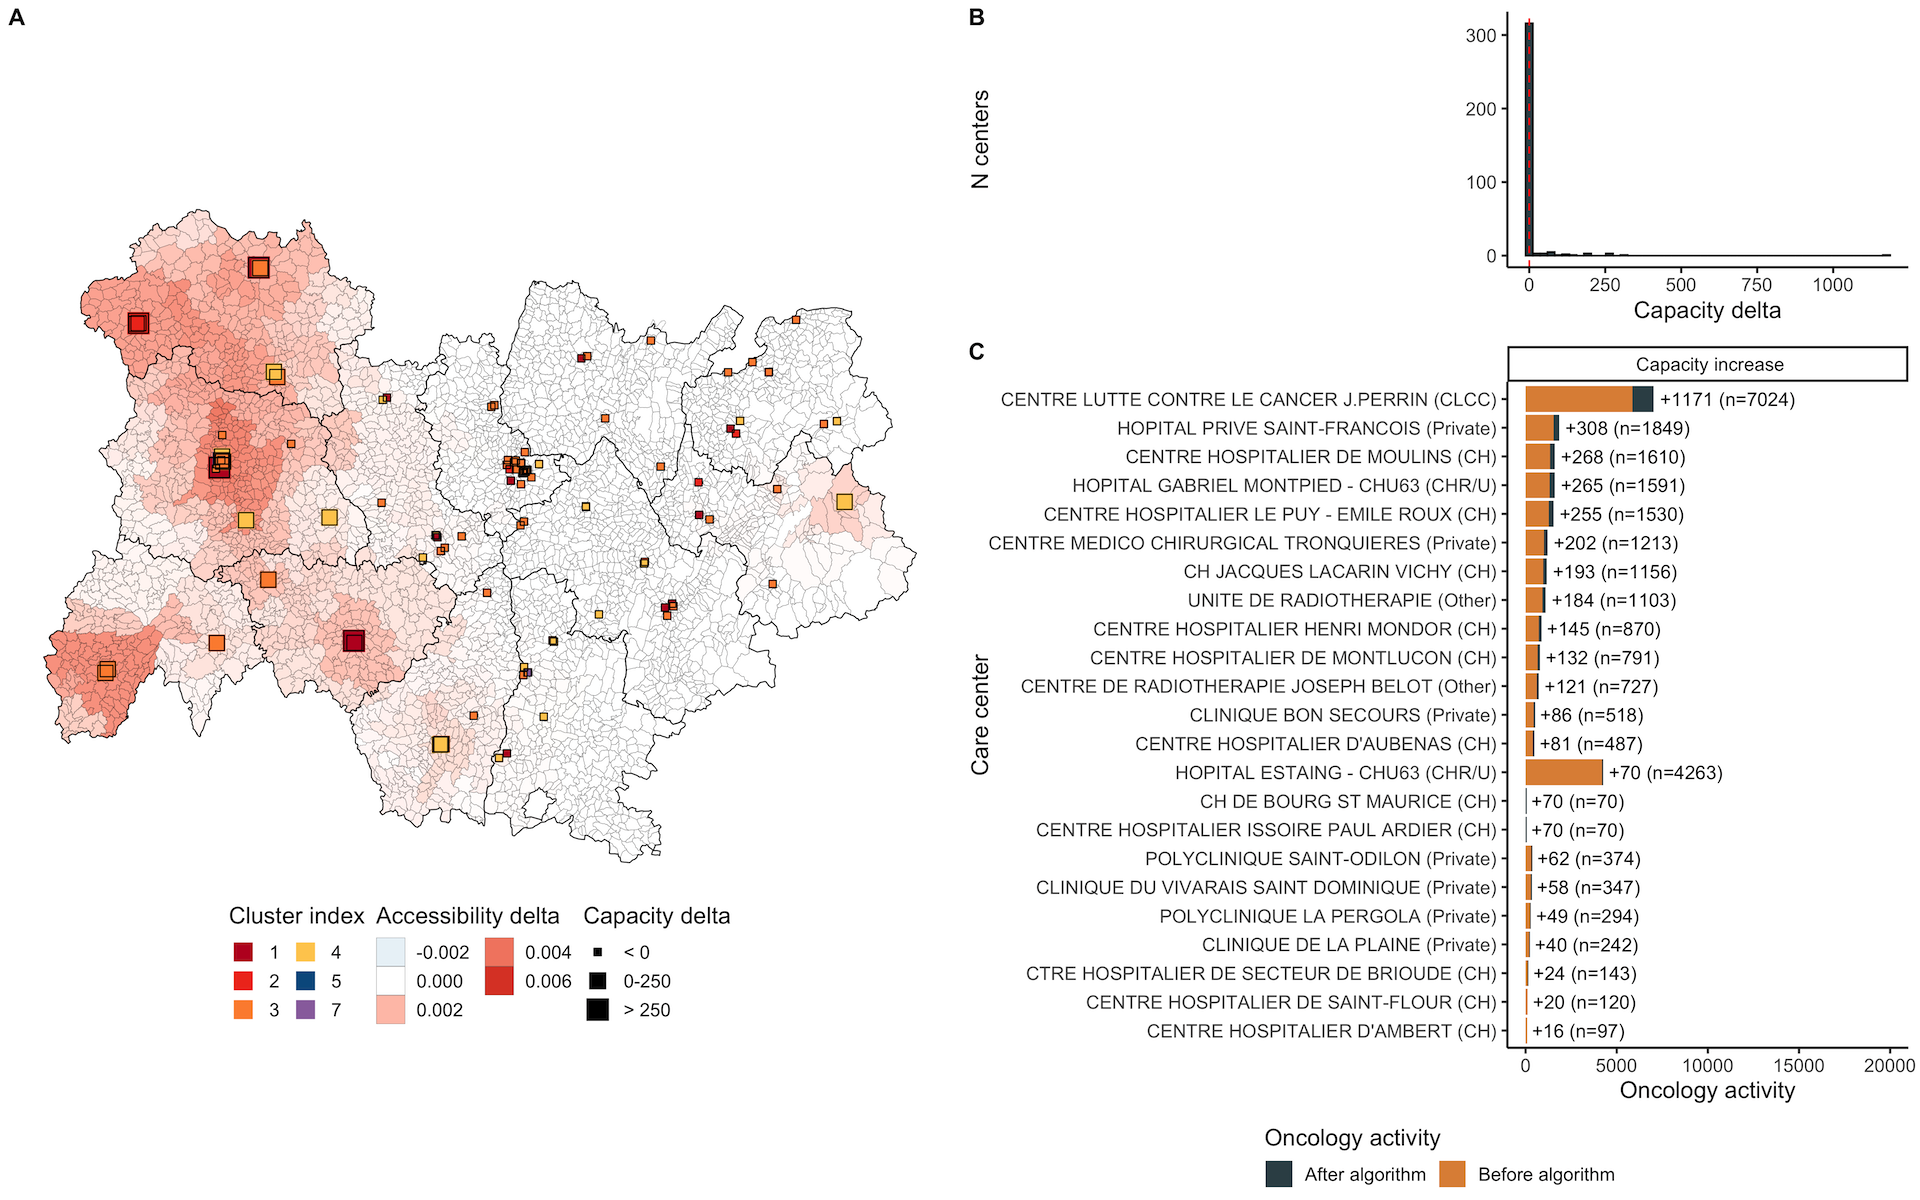
\includegraphics[width=0.9\textwidth]{images/camion/optim_region/optim_Auvergne-Rhone-Alpes.png}
    \centering
    \caption{
        \textbf{Optimization results in Auvergne-Rhone-Alpes.} Additional activity was 3,883. 23 centers grew and 2 decreased. Median accessibility before optimization was 0.0092 and 0.0095 after, corresponding to a 3.2\% increase. Accessibility grew around Moulins, Montluçon, Le Puy en Velay, Clermont-Ferrand and Aurillac.
    }
\end{figure}

\section{Web application}

We developed a web application that allows the users to run the optimization algorithm in any region with the parameters they want. The application displays accessibility results and optimization outcomes on an interactive map with additional plots. The user can browse the list of care centers by cluster and the list of municipalities with their accessibility scores.

\section{Open source code}

We open sourced the code for accessibility computation and \ac{camion} algorithm.
The code is available in the following Github repository: \url{https://github.com/ericdaat/CAMION}.

We applied our method to Health Facilities in New York City. We used datasets downloaded from NYC Open Data website, which lists free public data from New York City agencies and other partners. We downloaded the Zip Codes boundaries and census statistics in New York City, provided by the Department of Information Technology and Telecommunications. We retrieved the list of health facilities in the New York State, as well as their certifications for services and beds. Both datasets were provided by the New York State Department of Health. We only kept the health facilities located in New York City, with Medical / Surgical beds. Every hospital has Latitude / Longitude coordinates. We used Zip Codes polygons centroids as reference point to compute the travel between Zip Codes and hospitals. We used the Zip code population as $P_i$, to encode the demand variable. The supply variable $S_u$ was the number of Medical / Surgery bed for each Health Facility $u$. We used the geodesic (straight) distance between health facilities coordinates, and Zip Code centroid coordinates as distance matrix.

Download the datasets here:

\begin{itemize}
    \item \href{https://data.beta.nyc/dataset/nyc-zip-code-tabulation-areas/resource/894e9162-871c-4552-a09c-c6915d8783fb}{Zip Codes boundaries and census statistics in New York City}
    \item \href{https://health.data.ny.gov/Health/Health-Facility-General-Information/vn5v-hh5r}{List of health facilities in NY State}
    \item \href{https://health.data.ny.gov/Health/Health-Facility-Certification-Information/2g9y-7kqm}{Health facilities certifications for services and beds}
\end{itemize}

\begin{figure}[H]
    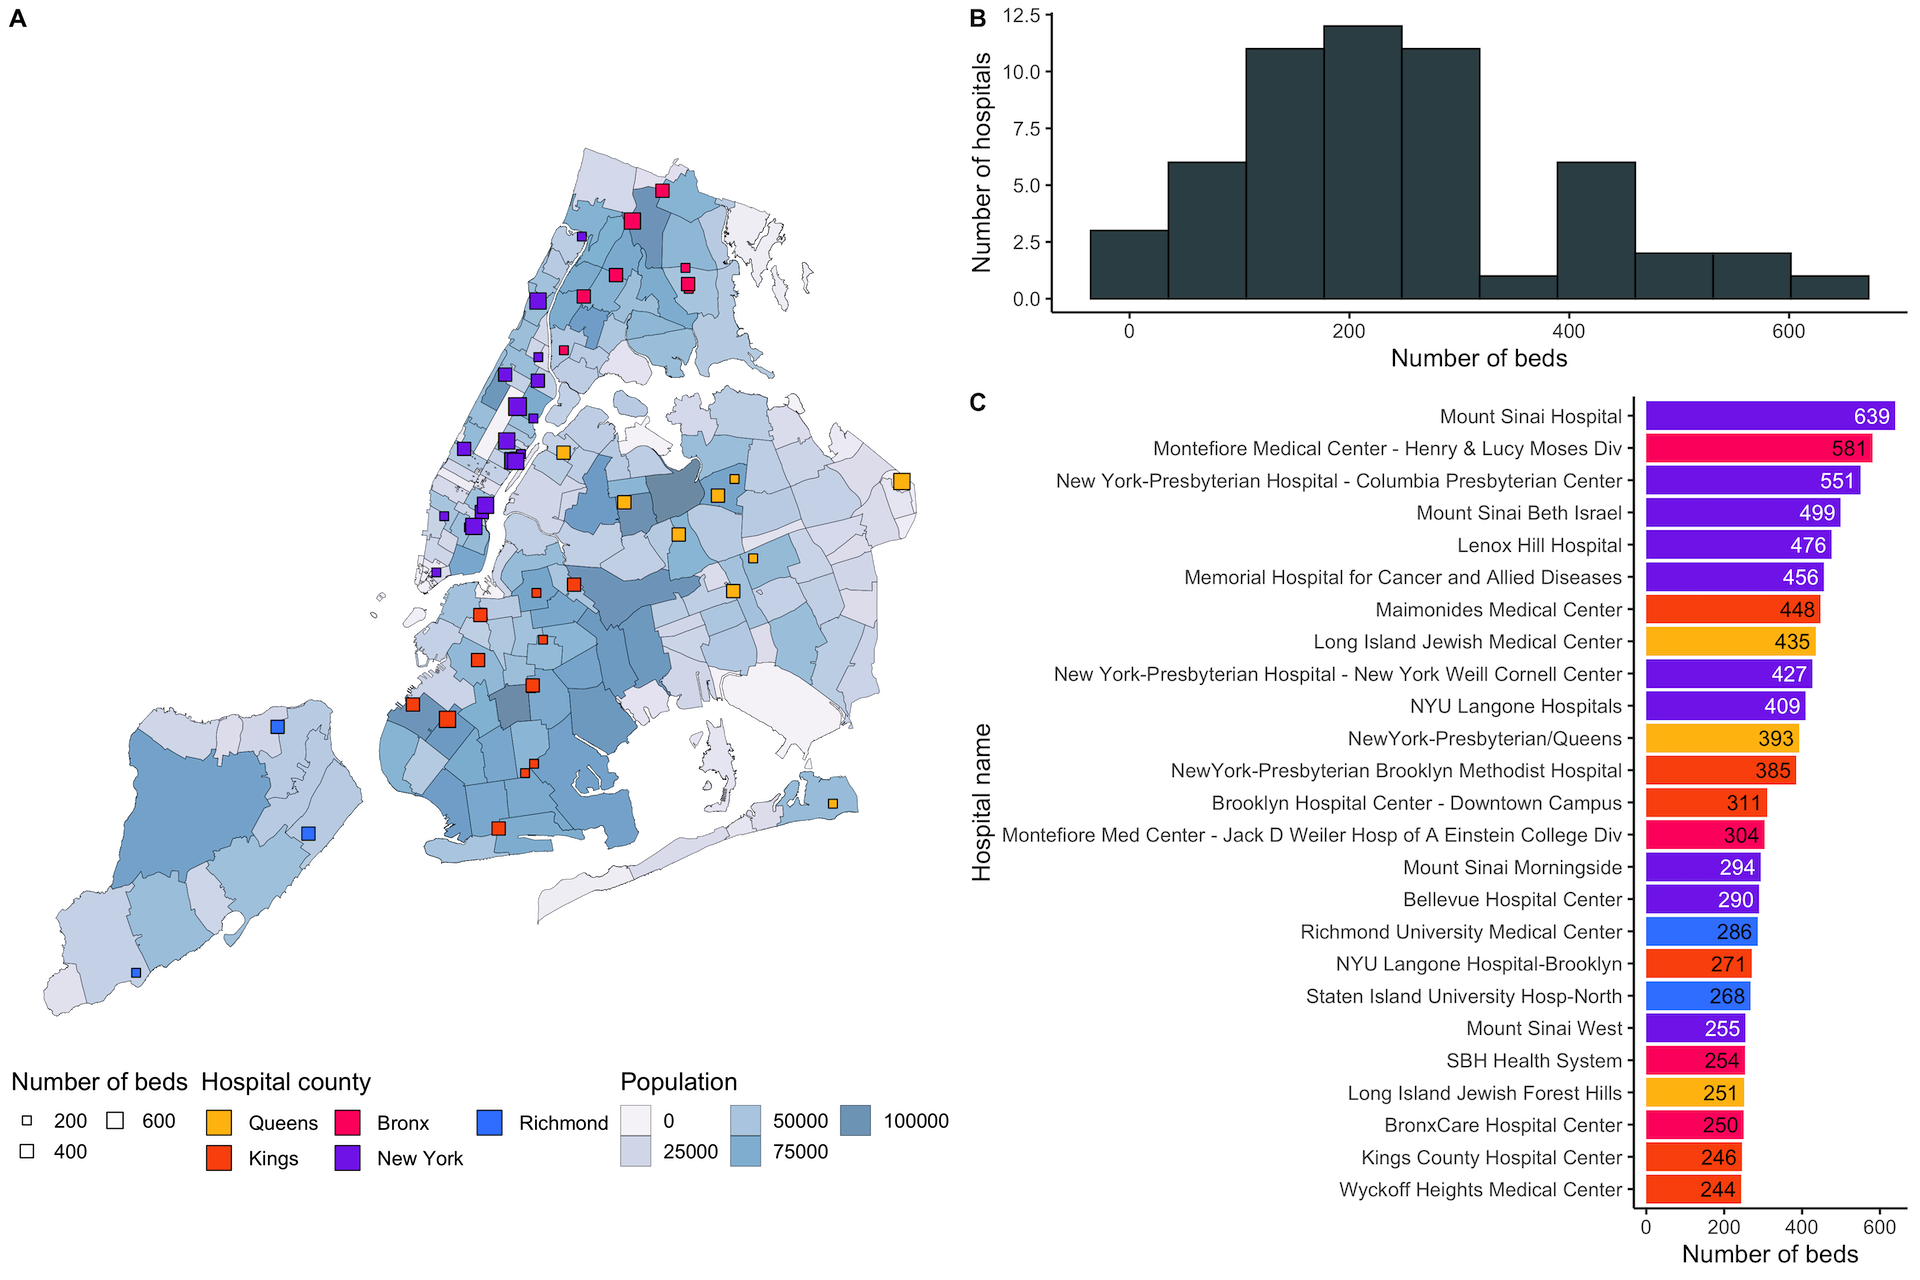
\includegraphics[width=0.9\textwidth]{images/camion-ny/fig1.png}
    \centering
    \caption{
        \textbf{Health facilities with Medical / Surgery beds in New York City.} We included 55 facilities with a total of 13,443 beds. Map (A) shows the geographical location of the facilities, colored by county, and sized by number of beds. The distribution of the number of beds is shown on (B). The top 30 facilities with the highest number of beds are listed on (C) and colored by county. The largest facilities are in New-York County.
    }
    \label{fig:camion-ny-beds}
\end{figure}

\begin{minipage}{\textwidth}
\begin{lstlisting}[language=Python, caption=Compute accessibility score with \ac{e2sfca}]
from camion.fca import E2SFCA

# Declare variables
P_i = np.random.rand(100)
S_j = np.random.rand(10)
D_ij = np.random.randint(low=1, high=100, size=(100, 10))

# Init E2SFCA algorithm
e2sfca = E2SFCA(
    S_j=S_j,   # Facilities
    P_i=P_i,   # Population locations
    D_ij=D_ij  # Travel impedance
)

# Choose weights for travel impedance
weights = [(30, 1), (60, 0.42), (90, 0.09)]

# Compute accessibility scores
A_i = e2sfca.compute_accessibility_score(weights)
\end{lstlisting}
\end{minipage}

\begin{figure}[H]
    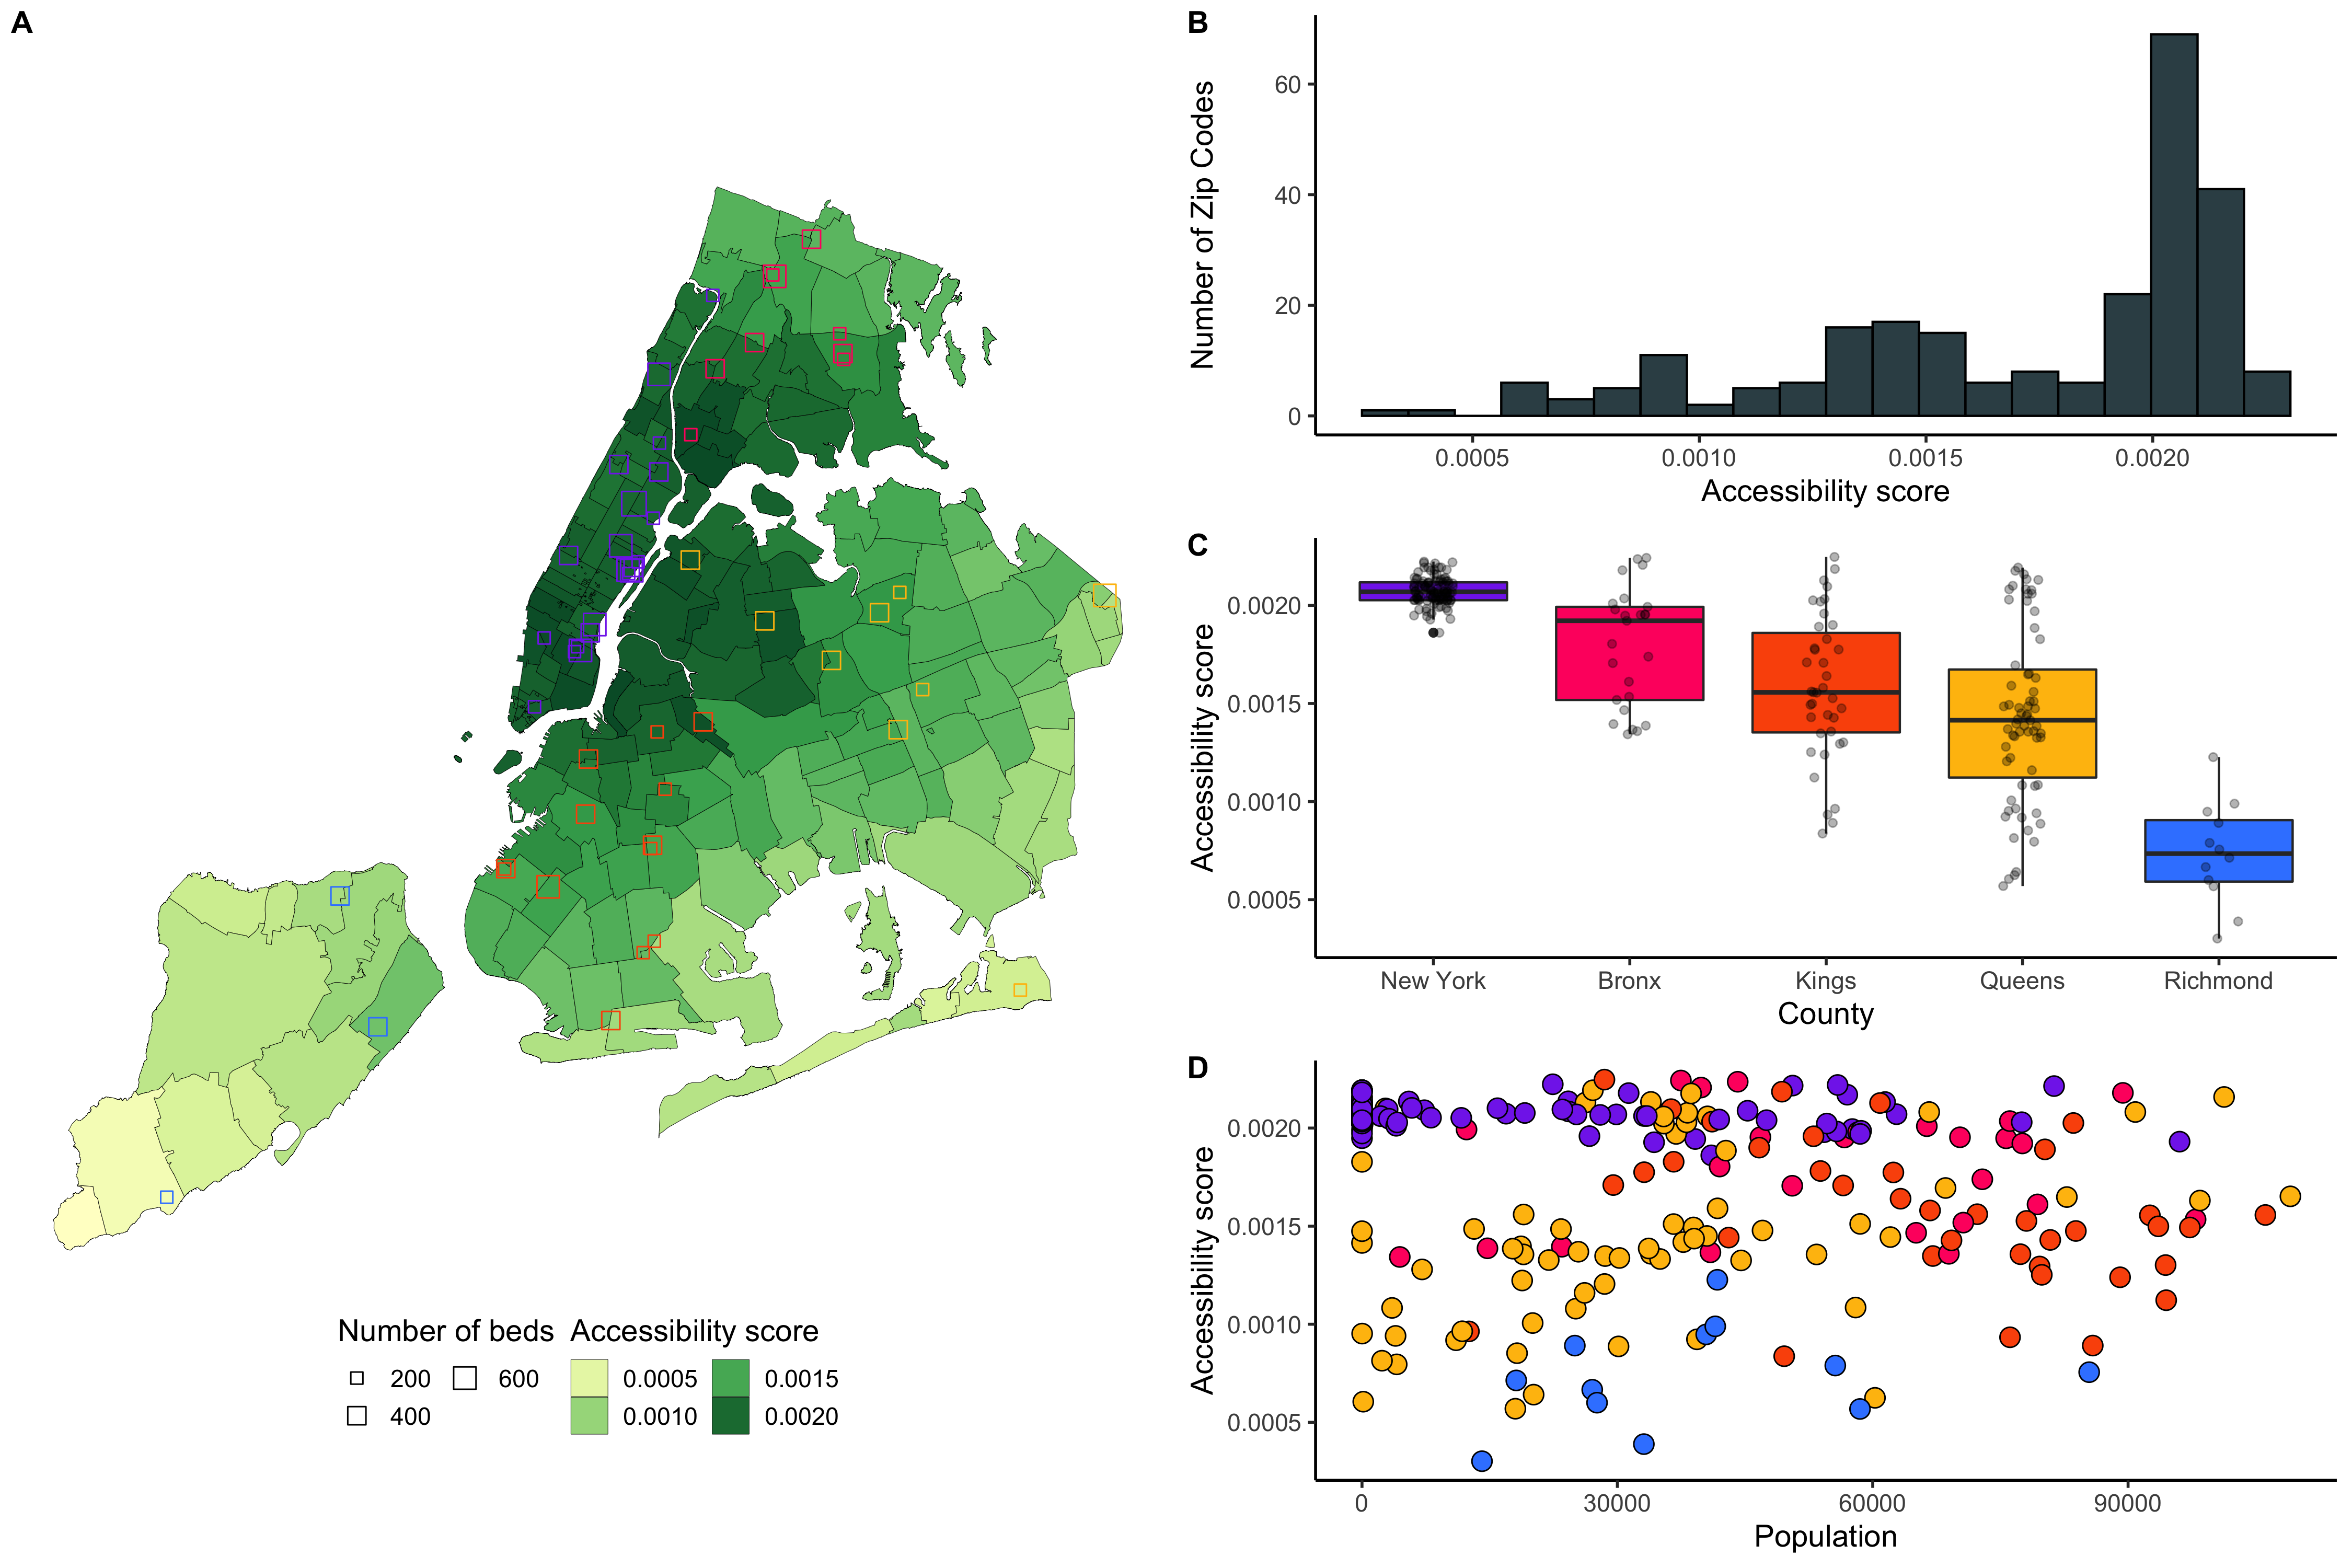
\includegraphics[width=0.9\textwidth]{images/camion-ny/fig2.png}
    \centering
    \caption{
        \textbf{Accessibility to Medical / Surgery beds in New York City.} Accessibility score was computed with the Enhanced Two Step Floating Catchment Area method, with a 45 km maximum catchment area. The geographical distribution of the accessibility score is shown on map (A). Zip codes are colored by accessibility score. Facilities are sized by number of beds and colored by county. The overall accessibility distribution is shown on (B). New-York County has the highest accessibility distribution where Richmond has the lowest (C). Accessibility seems to be higher in dense areas but there is no significant correlation between accessibility and population (D).
    }
    \label{fig:camion-ny-accessibility}
\end{figure}

\begin{minipage}{\textwidth}
\begin{lstlisting}[language=Python, caption=Optimize accessibility with \ac{camion}]
from camion.optimization import RegularOptimizer, MaxiMinOptimizer

# Define optimization parameters
budget = 1000
growth_percentage = 0.3

# Init regular optimizer
regular_optimizer = RegularOptimizer()

# Init maximin optimizer
maximin_optimizer = MaxiMinOptimizer()

# Run optimization with the optimization parameters
S_j_new_regular = regular_optimizer.run_optimization(
    S_j, P_i, W_ij,
    budget, growth_percentage
)

S_j_new_maximin = maximin_optimizer.run_optimization(
    S_j, P_i, W_ij,
    budget, growth_percentage
)
\end{lstlisting}
\end{minipage}

\begin{figure}[H]
    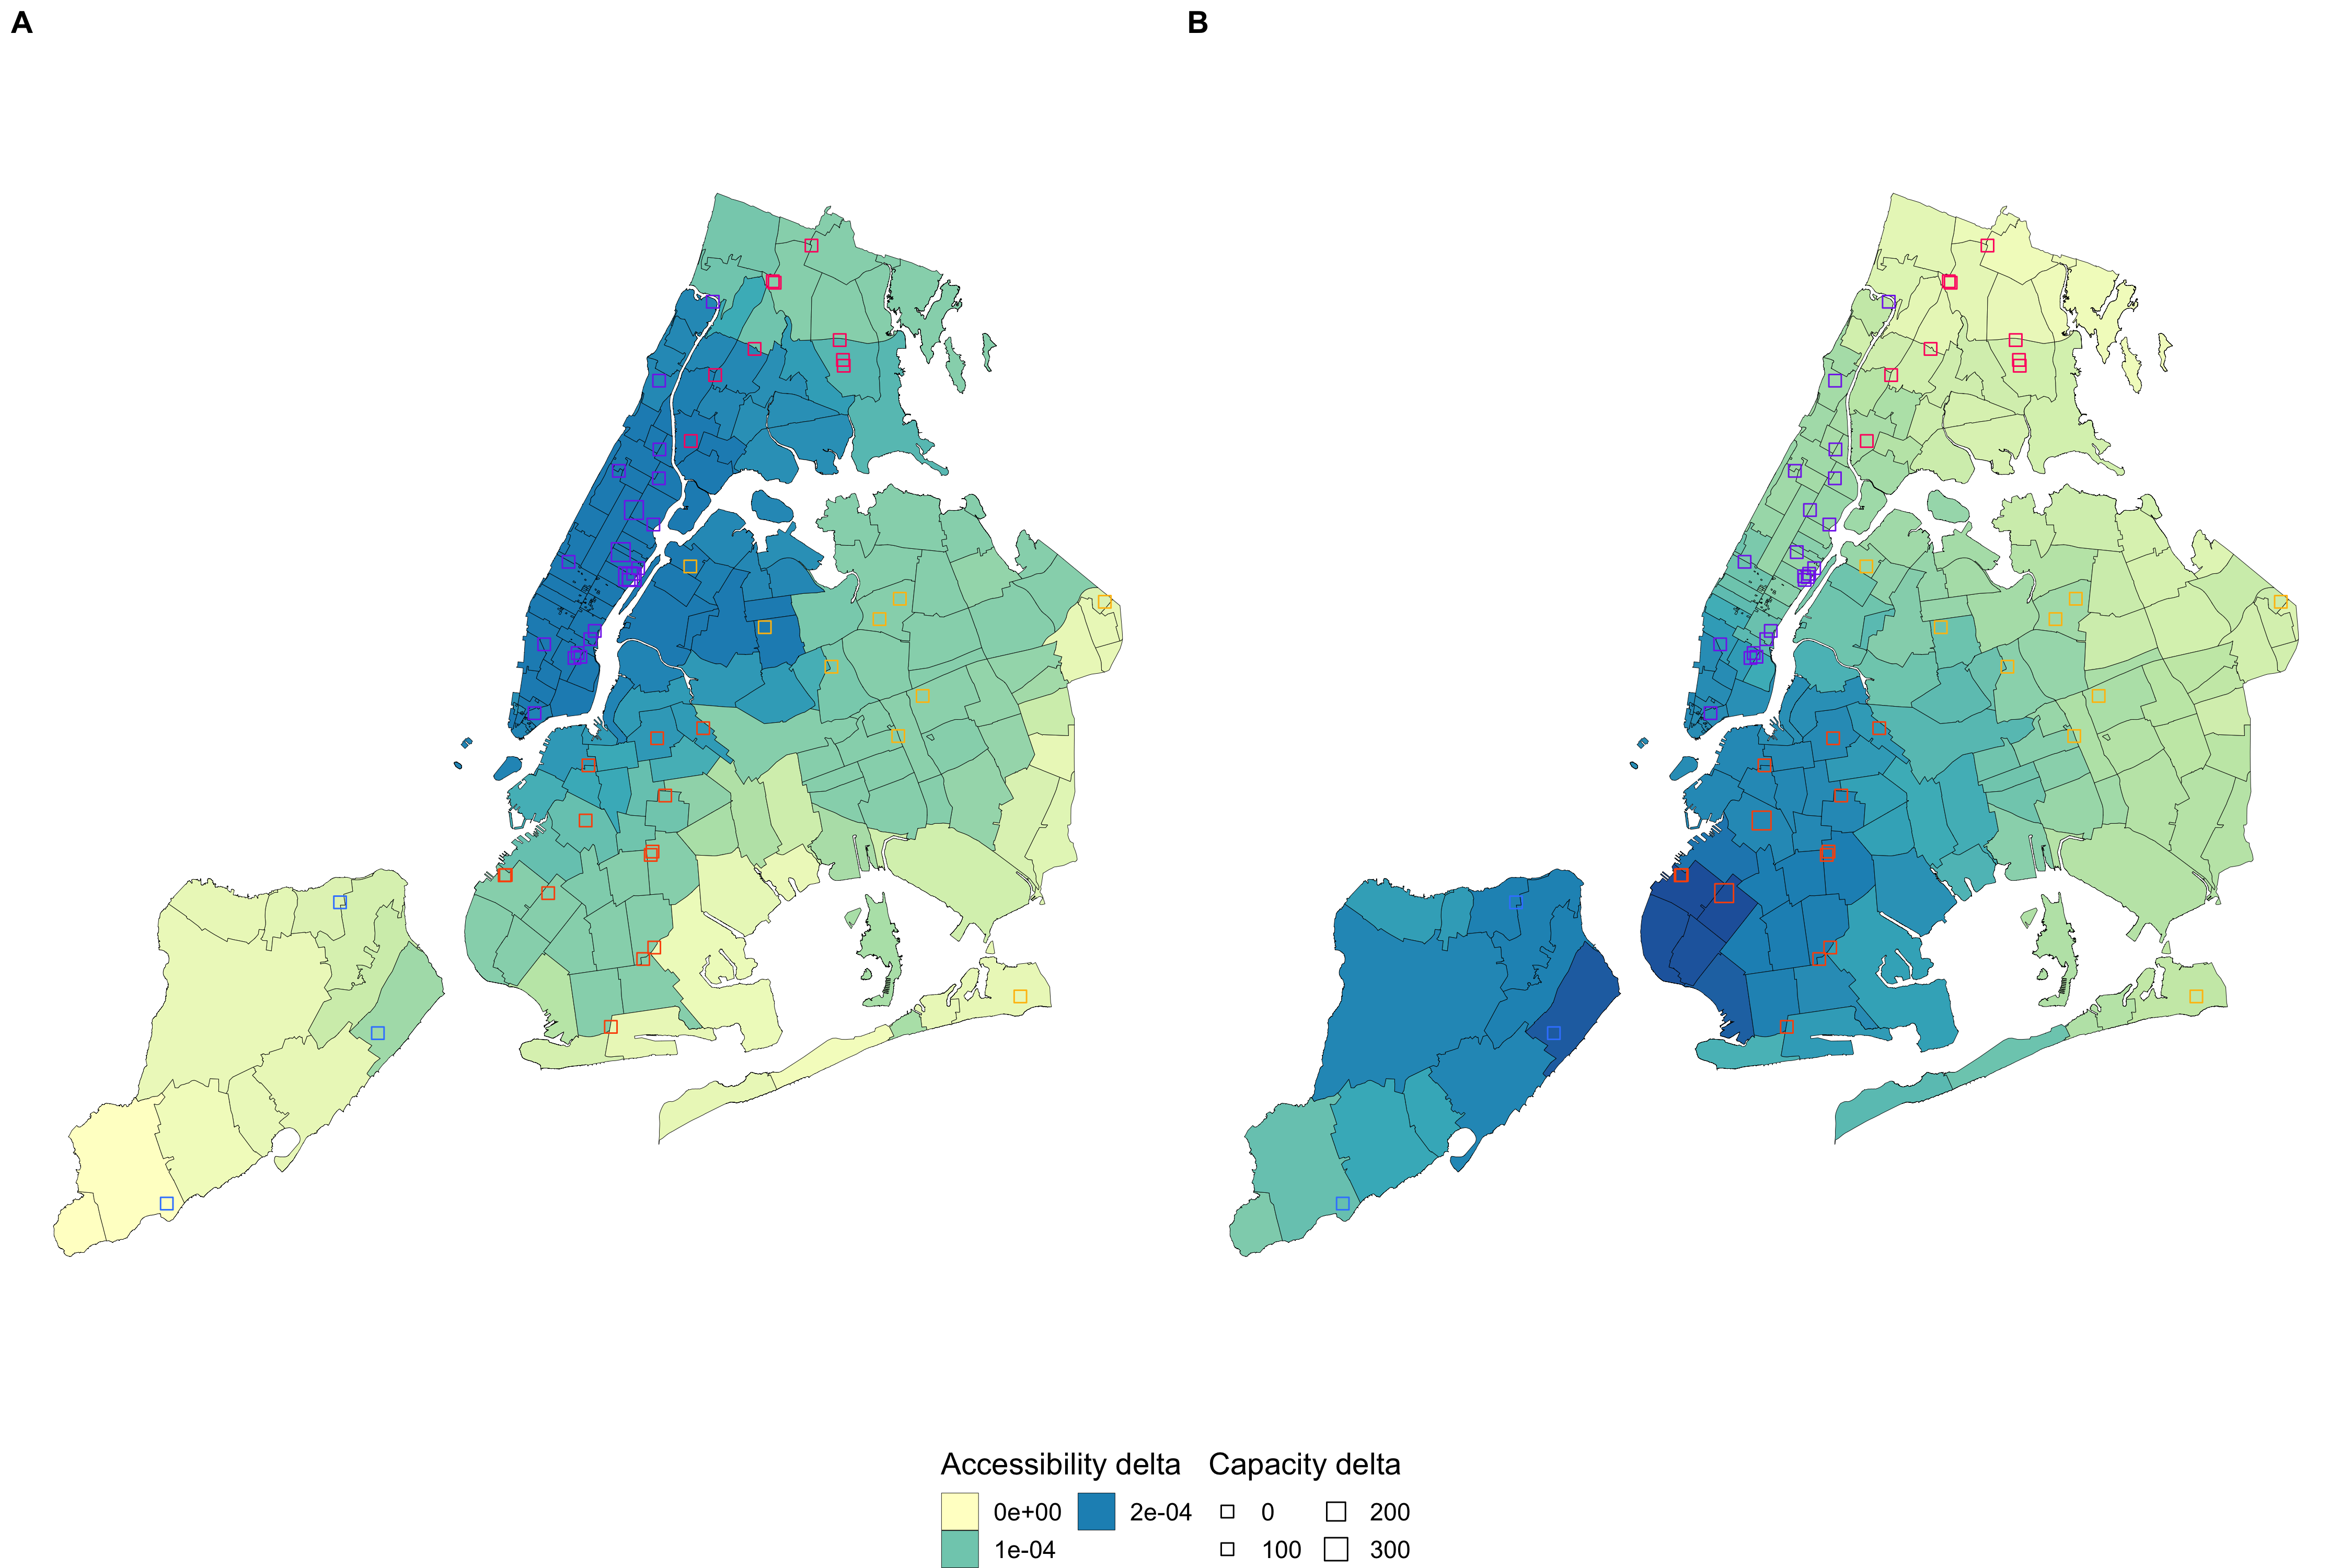
\includegraphics[width=0.9\textwidth]{images/camion-ny/fig3.png}
    \centering
    \caption{
        \textbf{Accessibility delta after running the optimization algorithm.}Both overall and maxi-min optimization algorithms are run. The optimization results are illustrated on maps (A) and (B) respectively. We displayed the accessibility delta as the difference of accessibility after and before the optimization. Every zip code is colored by accessibility delta. The health facilities are displayed as squares, sized accordingly to the capacity increase. The overall optimization increased facilities around New-York and Queens Counties (A). The maxi-min algorithm targeted Richmond facilities in priority (B).
    }
    \label{fig:camion-ny-optim}
\end{figure}

\section{Discussion}

The quality of oncology care is linked with the care centers' volume. A care center with a very low activity is less likely to provide decent care. As a result, \ac{inca} defined several thresholds (36) that forbid care centers with very low activity to keep operating. Similarly, the care quality in a saturated care center won't be good either, since patients are more likely to wait longer before diagnosis or between interventions. While it is easy to spot care centers with low activity, it is harder to judge if a care center is over-crowded, and we should be careful when attributing new activity to the hospitals. We based the 20\% max growth out of the previous centers’ activity increase. This percentage could be tailored to the center cluster or current activity. Volume is not the only factor determining care quality. More sophisticated indicators like average delay between diagnosis and first treatment can tell whether a care center is in line with the care pathways recommendations. Care centers with activities lower than the thresholds, or with a large proportion of degraded pathways should be handled with care by our algorithm.
Accessibility optimization depends on many factors and healthcare professionals will not have the same uses for our algorithm. Some may consider that for a care center to grow another should decline, where others would rather not decrease any centers' activities. Moreover, the healthcare planning is very different from a region to another, and even within the regions departments are showing disparities. Hence, we cannot expect the algorithm to be used with the same parameters on every region. For all these reasons, we believe that providing a web application to run the algorithm and choose the parameters is the most useful way to the help healthcare professionals improve the current situation.
